\documentclass[article,final,14pt]{scrreprt}
\usepackage[utf8x]{inputenc}
\usepackage[russian]{babel}
\usepackage{amsfonts}
\usepackage{enumerate}
\usepackage{amsthm}
\usepackage{amssymb}
\usepackage{vmargin}
\usepackage{amsmath}
\usepackage{graphicx}
\usepackage{listings}
\usepackage{color}
\usepackage{multicol}
\usepackage{pb-diagram}
% \usepackage[Lenny]{fncychap}
\usepackage{xcolor}
\usepackage{hyperref}
\setpapersize{A4}
\setmarginsrb{2cm}{1.5cm}{1cm}{1.5cm}{0pt}{0mm}{0pt}{13mm}
\usepackage{indentfirst}
\sloppy
\DeclareGraphicsExtensions{.pdf,.png,.jpg}
\graphicspath{{./ques/pics/}}

\definecolor{linkcolor}{HTML}{800000}
\definecolor{urlcolor}{HTML}{6495ED}

\hypersetup{pdfstartview=FitH,  linkcolor=linkcolor,urlcolor=urlcolor, colorlinks=true, pagecolor=linkcolor}

\setcounter{tocdepth}{2}
\linespread{1}
\begin{document}

\renewcommand\qedsymbol{$\blacksquare$}

\renewcommand\contentsname{Содержание}

\newtheorem{theorem}{Теорема}[chapter]

\newtheorem{problem}{Задача}[chapter]

\newtheorem{lemma}{Лемма}[chapter]

\newtheorem{clair}{Утверждение}[chapter]

\newtheorem{definition}{Определение}[chapter]

\newtheorem{property}{Свойство}[chapter]

\newtheorem{properties}{Свойства}[chapter]

\newtheorem{conseq}{Следствие}[chapter]

\newtheorem{remem}{Напоминание}[chapter]

\newtheorem{val}{Оценка}[chapter]

\newtheorem*{example}{Пример}

\newtheorem{fact}{Факт}[chapter]

\newtheorem*{mind}{Соображение}

\newtheorem*{mindanddef}{Соображения и определения}

\newtheorem*{remark}{Замечание}

\newtheorem*{notation}{Обозначение}

\newenvironment{Proof}       
	{\par\noindent{\bf Доказательство.}}
	{\hfill$\blacksquare$}

\newenvironment{solution}       
	{\par\noindent{\bf Решение.}}
	{\hfill$\blacksquare$}

\newcommand{\red}[1]{\textbf{\color{red}#1}}
\newcommand{\blue}[1]{\textbf{\color{blue}#1}}

\newcommand{\RNumb}[1]{\uppercase\expandafter{\romannumeral #1\relax}}

\def\ton#1{1,2,\dots,#1}
\def\Set#1#2{\left\{#1\colon#2\right\}}
\def\MYdef{\mathrel{\stackrel{\rm def}=}}
\def\QUdef{\mathrel{\stackrel{\rm ?}=}}
\def\pre#1{{}_{#1}}

\begin{titlepage}
  \begin{center}
    \large
 
  МОСКОВСКИЙ ГОСУДАРСТВЕННЫЙ УНИВЕРСИТЕТ ИМЕНИ М. В. ЛОМОНОСОВА 
    
    
\includegraphics[scale=0.6]{mm.jpg} 
     
    Механико-математический факультет
    \vspace{0.25cm} 
      
    экономический поток
    \vspace{0.8cm} 
     
    {\LARGE МАТЕМАТИЧЕСКИЕ МЕТОДЫ В ЭКОНОМИКЕ}
    
    \vspace{0.8cm} 
    4 курс

    \vspace{0.25cm} 
    7 семестр
\end{center}
\vfill
 
\newlength{\ML}
\settowidth{\ML}{«\underline{\hspace{0.7cm}}» \underline{\hspace{1cm}}}
\hfill\begin{minipage}{7cm}
  \begin{flushright}
    Лектор $\;\;$\\
    к. ф.-м. н., доцент $\;\;$
    И.М.~Никонов $\;\;$\\
    «\underline{\hspace{0.7cm}}» \underline{\hspace{2cm}} 2021 г. $\;\;$
  \end{flushright}
\end{minipage}%
\vfill
\bigskip
 
\begin{center}
  Москва, 2021 г.
\end{center}
\tikz[remember picture,overlay] \node[opacity=0.1,inner sep=0pt] at (8.5,12.5){
\includegraphics[scale=0.8]{background1}};
\clearpage
\end{titlepage}
\newpage

\begin{center}
	{\Large \textbf{Техническая информация}}
\end{center}

\vspace{0.5cm}
Данный PDF содержит примерную программу осеннего семестра 4 курса по предмету <<Математические методы в экономике>>.

\vspace{0.5cm}
Собрали и напечатали по мотивам лекций и семинаров студенты 4-го курса Конов Марк и Гащук Елизавета.

\vspace{0.5cm}
Авторы выражают огромную благодарность лектору, кандидату ф.-м. наук, доценту Никонову Игорю Михайловичу за прочитанный курс по предмету <<Математические методы в экономике>>.

\vspace{0.5cm}
Добавления и исправления принимаются на почты \href{}{vkonov2@yandex.ru} и \\\href{}{gashchuk2011@mail.ru}.

\vspace{0.5cm}
\begin{center}
	{\Large \textbf{ПРИЯТНОГО ИЗУЧЕНИЯ}}
\end{center}

\newpage



\tableofcontents



\chapter{Лекция №1 - 11.02.2021. Страхование жизни}\label{lec:1}


\begin{remark}
	Предполагается спокойное, мирное время. Страхование жизни основано на закономерностях уровня смертности различных групп населения.
\end{remark}

\section{Вероятность выживания} % (fold)
\label{lec:1sec:alive_prob}

Рассмотрим однородную группу людей. Время измеряем в годах.

\begin{definition}
	
	$x$ - возраст гражданина на момент заключения договора;

	$T_x$ - остаточное время жихни - случайная величина;

	$F(t) = P(T_x \leq t) \MYdef {}_{t}q_x$ - функция распределения $T_x$, обладающая плотностью распределения;

	$f(t)$ - плотность распределения $T_x$;

	${}_{t}p_x \MYdef P(T_x > t)$ - вероятность, что с момента $x$ человек проживет более $t$ лет;

	$\omega - x, $ - максимальное время жизни заключившего договор; $\omega$ обычно берут равным 100;
\end{definition}

\begin{definition}
	При заключении договора:
	\begin{enumerate}
		\item фиксируется продолжительность заболеваний страхователя;
		\item возраст страхователя;
	\end{enumerate}

	Тогда $\lambda$ - время, прошедшее между медицинским обследованием (началом заболевания) и началом страхования.
\end{definition}
	


\begin{clair}

	$${}_{\omega - x}p_x = 0.$$

	$${}_{0}p_x = 1.$$

\end{clair}

\begin{clair}

	Пусть 
	$${}_{\frac{t}{t'}}q_x \MYdef P(t < T_x \leq t + t').$$

	Тогда 
	$${}_{\frac{t}{t'}}q_x = {}_{t}p_x - {}_{t+t'}p_x > 0.$$

\end{clair}
\begin{Proof}

	$$P(T_x > t) = P(t \leq T_x \leq t+t') + P(T_x > t+t') \; \Rightarrow \; {}_{t}p_x = {}_{\frac{t}{t'}}q_x + {}_{t+t'}p_x. $$

\end{Proof}

\begin{conseq}
	Из доказательства очевидно вытекает
	\[ {}_{\frac{t}{t'}}q_x \;\rightarrow \; 0, \;\; t'\;\rightarrow\;0\]
\end{conseq}

\begin{definition}
	Рассмотрим $$P(t \leq T_x \leq t + \Delta t| T_x > t) = \frac{P(t < T_x \leq t + \Delta t)}{P(T_x > t)} $$

	Тогда $$\lim\limits_{\Delta t \rightarrow 0}\frac{P(t \leq T_x \leq t + \Delta t| T_x > t)}{\Delta t} = \lim\limits_{\Delta t \rightarrow 0}\frac{F(t + \Delta t) - F(t)}{\Delta t \pre{t}p_x} = \frac{f(t)}{1 - F(t)} \MYdef \mu_x(t)$$ называется \red{мгновенной смертностью в момент $x + t$} или \red{интенсивностью смерти}.
\end{definition}


\begin{properties}
	\begin{enumerate}
		\item $\mu_x(t) \geq 0 $ при $t \in [0, \omega - x]$
		\item $\int\limits_0^b\mu_x(t)dt = \infty$, где $b > \omega - x$
	\end{enumerate}
\end{properties}

\begin{remark}
	\begin{gather*}
		\mu_x(t) = \frac{F'(t)}{1-F(t)} = \frac{-\frac{\partial}{\partial t}(1-F(t))}{1-F(t)}
		= \frac{-\frac{\partial}{\partial t}(\pre{t}p_x)}{\pre{t}p_x} = -\frac{d}{dt}\ln\pre{t}p_x
	\end{gather*}
		
	

	\[\Rightarrow \pre{t} p_x = e^{-\int\limits_0^t\mu_x(u)du}\]
\end{remark}


\section{Модели смертности} % (fold)
\label{lec:1sec:death_mod}

\begin{description}
	\item[\blue{Муавр}] \begin{gather*}
		T_x[0, \omega - x] - \text{равномерно распределена}\\
		f(t) = \begin{cases}
			\frac{1}{\omega - x}, 0 \leq t \leq \omega-x\\
			0, else
		\end{cases}
		\end{gather*}
	\item[\blue{Гомпретц}]
		\[\mu_x(t) = AC^{x+t}, (A>0, C>1)
		\]
		Отсюда $$\pre{t}p_x \rightarrow 0 (t \rightarrow \infty)$$

	\item[\blue{Мэйкхэм}]
		\[\mu_x(t) =D+ AC^{x+t}, (A>0, C>1, D>0)
		\]
		Тут берётся во внимние тот факт, что смерть может наступать не только от старости.

		\[
		{}_tp_x = e^{-\int\limits_0^tD+AC^{x+t}} = e^{-Dt - \frac{A(C^{x+t} - C^x)}{\ln C}}
		\]

	
\end{description}

\section{Оценка числа людей, доживших до момента t}
\label{lec:1sec:eval}

Пусть
\[
L_x- \text{\red{число людей возраста х из однородной группы}.}\]

Выбираем людей тщательно, ибо время считается в годах.


Определим индикатор
\[
X_i(t) = \begin{cases}
	1, i-\text{ый человек проживет больше, чем}t\\
	0, \; \;else
	
\end{cases}
\]

Тогда

\begin{gather*}
	EX_i(t) = {}_tp_x \\
	DX_i(t) = {}_tp_x - ({}_tp_x)^2 = {}_tp_x{}_tq_x.
\end{gather*}

Положим

\[
L_{x+t} \MYdef X_1(t) +...+ X_{L_x}(t) \]

Тогда

\begin{gather*}
	EL_{x+t} = L_x{}_tp_x \MYdef l_{x+t}\;\;(\Rightarrow EL_x = L_x)\\
	DL_{x+t} = L_x{}_tp_x{}_tq_x\;\text{(в силу независимости смертей)}.
\end{gather*}

\begin{remark}
	Видно, что \[{}_tp_x = \frac{l_{x+t}}{l_x} \]
\end{remark}
\chapter{Лекция №2 - 18.02.2021}\label{lec:2} % (fold)

\section{Оценка числа доживших до момента t} % (fold)

Используя обозначения прошлой лекции, имеем

\begin{clair}
	$ l_{\omega + \varepsilon } = 0, \;\;\; l_{x+t} = l_y(x \leq y \leq \omega) = l_x {}_tp_x $
\end{clair}

Множество значений $ l_y$ определяет \red{закон выживаемости}. По нему строится \red{таблица смертности}. При этом обычно берутся $ l_x \sim 10^5, 10^6.$

\section{Ожидаемая продолжительность оставшейся длительности жизни} 
\label{sec:expectd}


\begin{definition}
	\red{Ожидаемой продолжительностью оставшейся длительности жизни} называется математиеческое ожидание дожития $\mathring{e}_x=ET_x$
\end{definition}

Имеем
\begin{gather*}
	\mathring{e}_x = \int\limits^{\omega - x}_{0}tf(t)dt = \int\limits^{\omega - x}_{0}tF'(t)dt = -\int\limits^{\omega - x}_{0}t(1-F(t))'dt =\\
	=[0\leq T_x \leq \omega - x] = -\int\limits^{\omega - x}_{0}t({}_tp_x)'dt = -\int\limits^{\omega - x}_{0}t(\frac{l_{x+t}}{l_x})'dt = -\frac{1}{l_x}-\int\limits^{\omega - x}_{0}t(l_{x+t})'dt=\\
	=[d(tl_{x+t}) = tl'_{x+t}dt + l_{x+t}dt] = -\frac{1}{l_x}\int\limits^{\omega - x}_{0}d(tl_{x+t}) + \frac{1}{l_x}\int\limits^{\omega - x}_{0}l_{x+t}dt=\\
	=\frac{1}{l_x}\int\limits^{\omega - x}_{0}l_{x+t}dt = \frac{1}{l_x}\int\limits^{\omega}_{x}l_ydy
\end{gather*}

\begin{val}
Оценим полученный интеграл:
	\begin{gather*}
		\sum\limits^{\omega - x -1}_{k = 0}l_{x+k+1} < \int\limits^{\omega}_{x}l_ydy < \sum\limits^{\omega - x -1}_{k=0}l_{x+k}\\
		\frac{l_{x+1}+...+l_{\omega}}{l_x} < \frac{1}{l_x}\int\limits^{\omega}_{x}l_ydy < 1 + \frac{l_{x+1}+...+l_{\omega}}{l_x}\\
		e_x < \mathring{e}_x < 1 + e_x,\\
		 \text{ где } e_x \text{ \red{усечённая ожидаемая продолжительность оставшейся жизни}}\\
		\mathring{e}_x \approx \frac{1}{2} + e_x
	\end{gather*}
\end{val}

\begin{definition}
	Пусть имеем начальное число индивидов в возрасте 0 лет ( можно любое другое число лет) $ l_0 = L_0$.

	Тогда 
	\begin{gather*}
		l_1 = l_0(1-q_0)\\
		l_2 = l_1(1-q_1)\\
		...\\
		l_{x+1}=l_x(1-q_x)
	\end{gather*}

	Введем 
	\[\overline{X}_i=
		\begin{cases}
			0, \; p_x - \text{ прожил больше года}\\
			1, \; q_x - \text{ скончался в течение года}
		\end{cases}
	\]
	и 
	\[
		D_x = \sum\limits^{L_x}_{i=1}\overline{X}_i
	\]

	Тогда величина
	\[Q_x = \frac{D_x}{L_x}\]
	называется \red{коэффициентом наблюдаемой годовой смертности}.
\end{definition}

\begin{clair}
Имеем
	\begin{gather*}
		EQ_x = \frac{ED_x}{L_x} = \frac{L_xq_x}{L_x} = q_x\\
		DQ_x = \frac{DD_x}{L_x} = \frac{\sum D\overline{X}_i}{L^2_x} = \frac{q_xp_x}{L_x}
	\end{gather*}
ввиду независимости $ \overline{X}_i $. 
\end{clair}

Рассмотрим величину

\[ \frac{Q_x - q_x}{\sqrt{DQ_x}}.\]

При больших значениях $ L_x$ распределение данной величины близко к стандартному нормальному в силу ЦПТ. Тогда
\[ P(\frac{|Q_x - q_x|T_x}{\sqrt{p_xq_x}} < t) = 2\Phi(t) -1, \]
где $ \Phi(t)-$ функция распределения стандартного нормального распределения.

\begin{example}
	Пусть 
	\begin{gather*}
		t = 2\;\;\; \Rightarrow \;\;\; \Phi(2) = 0,9772\\
		L_x = 100000\\
		D_x = 261\\
		\Rightarrow\;\;\; Q_x = \frac{261}{100000} = 0,0261
	\end{gather*}
	Однако на деле имеем
	\begin{gather*}
		p_x \approx 1\\
		q_x \approx Q_x\\
		\Rightarrow \;\;\; Q_x - 2 \sqrt{\frac{Q_x}{L_x}} < q_x < Q_x + 2\sqrt{\frac{Q_x}{L_x}}\\
		\Rightarrow\;\;\; 2,281 < q_x < 2,933 permill
	\end{gather*}
\end{example}

ТУТ ТАБЛИЦА СМЕРТНОСТИ ПО АНГЛИИ

\begin{clair}
	Для непересекающихся прожеутков времени имеем
	\[{}_{x+t}p_0 = {}_xp_0{}_tp_x	\]
\end{clair}

\begin{proof}
	\begin{gather*}
		{}_tp_x = P(T_x > t) = P(T_x + x > x+t) = P(T_0 > t+x|T_0 > x)=\\
		=\frac{P(T_o > t+x)}{P(T_0>x)}=\frac{{}_{t+x}p_0}{{}_{x}p_0}
	\end{gather*}
\end{proof}

Можем строить \red{таблицы смертности}. Бывают \red{полные, неполные, селективные} таблицы.

Пусть
\[[x]-\text{ время заключения договора при одновременном прохождении медосмотра}\]

\[	P_{[x]}- \text{ вероятность прожить год с момента х.}\]

Имеет место эмпирический

\begin{fact}
	\begin{gather*}
		p_{[x]} > p_{[x-1]+1} > p_{[x-2]+2}>...\\
		p_{[x-r]+r}=p_{[x-r-1]+r+1} = ...,
	\end{gather*}
	где $ r$ - \red{период отбора(время селекции)} = 5-7 лет
	
\end{fact}

\chapter{Лекция №2 - 18.02.2021. Дожитие как сумма целой и дробной частей} % (fold)
Имеем
\[	T_x \equiv T(x) = K(x) + S(x) ,\]

где 
\begin{gather*}
	T_x - \text{ случайная величина - время жизни, начиная с х лет}\\
	K(x) = [T_x] - \text{ целая часть от времени жизни - случайная величина}\\
	S(x) = \{T_x\} - \text{ дробная часть от времени жизни - случайная величина}
\end{gather*}

\section{Распределение и моменты K(x)} % (fold)

\begin{theorem}
	\begin{gather*}
		P(K(x) = k) = {}_kp_x - {}_{k+1}p_x\\
		EK(x) = \sum\limits^{\infty}_{k = 1}{}_kp_x = e_x\\
		DK(x) = \sum\limits^{\infty}_{k=1}{}_kp_x(2k-1) - (\sum\limits^{\infty}_{k=1}{}_kp_x)^2
	\end{gather*}
	
\end{theorem}

\begin{proof}
	Непосредственно следуя определениям, выпишем распределение и математическое ожидание $ K(x)$:
	\begin{gather*}
		P(K(x) = k) = P(k \leq K(x) \leq k+1) = {}_kp_xq_{x+k} = {}_kp_x(1 - p_{x+k}) = \\
		={}_kp_x - {}_kp_xp_{x+k} = {}_kp_x - {}_{k+1}p_x\\
		EK(x) = \sum\limits^{\infty}_{k=1}kP(K(x) = k) = \sum\limits^{\infty}_{k=1}k({}_kp_x - {}_{k+1}p_x) =\\
		= \sum\limits^{\infty}_{k=1}{}_kp_x - {}_{k+1}p_x + \sum\limits^{\infty}_{k=2}{}_kp_x - {}_{k+1}p_x + ...==\\
		= [p_x - {}_2p_x + {}_2p_x - {}_3p_x + ...] + [{}_2p_x - {}_3p_x +{}_3p_x - {}_4p_x + ...] = \sum\limits^{\infty}_{k = 1}{}_kp_x = e_x
	\end{gather*}
	Для подсчета дисперсии по определению
	\[DK(x) = E(K(x))^2 - (EK(x))^2 \]

	воспользуемся слеудющим соображением:
	\begin{mind}[\blue{Суммирование по частям}]
		Пусть \[\Delta f_k = f_{k+1} - f_k. \]
		Тогда \[ \sum\limits^{b}_{k=a}\Delta f_a + \Delta f_{a+1} + ...+ \Delta f_b = f_{b+1} - f_a = f_k|^{b+1}_a. \]

		Также 
		\begin{gather*}
			\Delta u_kv_k = u_{k+1}v_{k+1} - u_kv_k = u_{k+1}v_{k+1}- u_{k+1}v_k - u_kv_k=\\
			u_{k+1}\Delta v_k + v_k\Delta u_k.
		\end{gather*}

		Отсюда
		\begin{gather*}
			\sum\limits_{k=a}^{b} \Delta(u_kv_k) = u_kv_k|^{b+1}_a = \sum\limits_{k=a}^{b}u_{k+1}\Delta v_k + \sum\limits_{k=a}^{b}v_k\Delta u_k\\
			\Rightarrow\;\;\; \sum\limits_{k=a}^{b}v_k\Delta u_k = u_kv_k|^{b+1}_a - \sum\limits_{k=a}^{b}u_{k+1}\Delta v_k
		\end{gather*}
	\end{mind}

	Согласно соображению
	\begin{gather*}
		E(K(x))^2 = \sum\limits_{k=0}^{\infty}k^2({}_kp_x - {k+1}p_x) =\\
		= -{}_kp_xk^2|^{\infty}_0 + \sum\limits_{k=0}^{\infty}{}_{k+1}p_x(2k +1)=[\lim\limits_{k\rightarrow \infty}{}_kp_x = 0] = \sum\limits_{r=1}^{\infty}{}_rp_x(2r-1)\\
		\Rightarrow \;\;\; DK(x) = \sum\limits_{k=1}^{\infty}{}_kp_x(2k-1) - (\sum\limits_{k=1}^{\infty}{}_kp_x)^2	
	\end{gather*}
\end{proof}
% section распределение_и_моменты_k (end)

\section{Распределение и моменты S(x)}

Рассмотрим 3 варианта моделей
\begin{enumerate}
	\item \red{Линейная модель} $ \Leftrightarrow \;\;\; {}_uq_x = uq_x, \;\;\; u \in [0;1)$

			\begin{theorem}
				$ S(x)$ равномерно распределена.
			\end{theorem}
			\begin{conseq}
			\begin{gather*}
				ES(x) = \frac{1}{2}\\
				DS(x) = \frac{1}{12}\\
				\mathring{e}_x = ET(x) =\frac{1}{2} + e_x\\
				DT(x) = DK(x) + \frac{1}{12}
			\end{gather*}	
			\end{conseq}
			\begin{proof}
				Найдем распределение:
				\begin{gather*}
					P(S(x) \leq u| K(x) = K) = \frac{{}_uq_{x+k}}{q_{x+k}} = \frac{uq_{x+k}}{q_{x+k}} = u\\
					S(x), K(x) - \text{ независимы } \Rightarrow\;\;\; P(S(x) \leq u) = u
				\end{gather*}
			\end{proof}
			\begin{remem}
			 Помним:
				  \[ \mu _x(u) - \text{ \red{интенсивность смерти} }, \]
			также
				\begin{gather*}
				 	{}_tp_x = e^{-\int\limits^{t}_{0}\mu(u)du}\\
				 	\Rightarrow\;\;\; \mu_x(u) = -\frac{d\ln({}_up_x)}{du} = -\frac{d\ln(1- {}_uq_x)}{du} = \\
				 	=-\frac{1 - uq_x}{du} - \text{ монотонно возрастающая функция u}.
				\end{gather*}  
			\end{remem}
	\item \red{Постоянство интенсивности смерти в течении года}
		\[
			\forall \;\;u \in [0;1) \;\;\; \mu_k(u) = \mu_k(\frac{1}{2}) = \mu_{k+\frac{1}{2}},
		\]
		т.е. интенсивность смерти приближают ступенчатой функцией. Отсюда
		\[	{}_tp_x = (p_x)^t	\]
		и
		\begin{gather*}
			P(S(x) \leq u | K(x) = k)= \frac{{}_uq_{x+k}}{q_{x+k}} = \frac{1-(p_{x+k})^u}{1-p_{x+k}}
		\end{gather*}
		Понятно, как считать моменты.
		\begin{remark}
			 В такой модели не может быть независимости между $ K(x) \text{ и } S(x)$
		\end{remark}

	\item \red{Условия Балдуччи}:

	\[ \forall\;\; u \in [0;1) \text { имеем } {}_{1-u}q_{x+u} = (1-u)q_x \]

	\begin{remark}
		Имеем для первого типа модели
		\[ {}_{1-u}q_x = (1-u)q_x. \]
		А для данной
		\[ {}_{1-u}q_{x+u} = (1-u)q_x.\]
		Но
		\[  {}_{1-u}q_x \neq {}_{1-u}q_{x+u},\]
		А значит 1 модель точно не совпадает с 3.
	\end{remark}
	\begin{mind}
		Вероятность прожить год:
		\[	p_x = {}_up_x{}_{1-u}p_{x+u}\;\;\;\Rightarrow\;\;\; {}_up_x = \frac{1-q_x}{1-(1-u)q_x}.\]
		С другой стороны
		\[  {}_tp_x = e^{-\int\limits^{t}_{0}\mu_x(u)du} .\]
		Значит
		\[  \mu_x(u) = \frac{q_x}{1-(1-u)q_x} \]
	\end{mind}

	\blue{Распределение дробной части} в данной модели
	\begin{gather*}
		P(S(x) \leq u| K(x)=k) = \frac{{}_kp_x{}_uq_{x+k}}{{}_kp_xq_{x+k}}=\\
		=[q_{x+k} \text{ можно записать: } ] = \frac{u}{1-(1-u)q_x}
	\end{gather*}

	\begin{remark}
		$ \mu_x(u)$ на интервале внутри года по этой модели монотонно убывает, что противоречит действительности.
	\end{remark}
\end{enumerate}



\chapter{Лекция №2 - 18.02.2021. Долгосрочные финансовые операции} 
\section{Вводные слова} % (fold)


% section вводные_слова (end)
Деньги приносят доход. Он зависит от
\begin{enumerate}
	\item времени
	\item начальной суммы
	\item процента дохода
\end{enumerate}

Пусть в начале клиент платит страховой компании $ Z$ рублей.

В момент смерти компания выплачивает $ Y$ рублей.

Пока говорим о целом числе лет.

\begin{mindanddef}
	Пусть $ i$ - \red{процентная ставка} (доля годового роста капитала).

	$ v = \frac{1}{1+i} -  $ \red{дисконтирующий множитель}.

	Пусть клиент умрет через $ T$ лет.

	Через $ T$ лет сумме $ Z$ соответствует сумма $ Z(1+i)^T.$

	В момент $ t = 0$ (\red{момент заключения контракта}) финансовые обязанности клиента: \[ Z, \]
	страховой компании: \[ Y(1+i)^{-T}, \]
	где $ Z = Y(1+i)^{-T} - $ \red{ настоящее значение $Y$ (present value)} ($pvY$).

	Но в долгосрочном страховании $ Z, i , Y - $ константы, а $ T -$ случайная величина с функцией распределения $ F(t)$ и плотностью распределения $ f(t) = \frac{dF(t)}{dt} $.

	Тогда 

	\begin{gather*}
		E(pvY) = Y \int\limits^{\infty}_{0}(1+i)^tf(t)dt\\
		D(pvY) = [E(pvY)^2] - [E(pvY)]^2 = Y^2 \int\limits^{\infty}_{0}(1+i)^{-2t}f(t)dt - [E(pvY)]^2.
	\end{gather*}

	Естественно, что в качестве премии выбирают не $ Y(1-i)^{-T}$, а 
	\[ \pi = E(pvY)= EZ \]
	- \red{ одноразовая нетто ставка}.

\end{mindanddef}

\section{Дисконтированные платежи} % (fold)
Для предпринимателя (банк, страховое общество), получающего и выдающего денежные суммы в разное время, важно на какой срок приходит к нему или уходит от него некоторая сумма. От пришедшей суммы предприниматель может получить некторый доход, а от выданной суммы теряется возможный доход. Для сравнения сумм, поступающих или уходящих в разное время вводится понятие \red{ современной дисконтированной стоимости платежа}.

\begin{mindanddef}
	Пусть $ A(t)$ - \red{ функция накопления}
	\[ A(t) = A(0)(1+i)^t, \]
	где $ A(0)$ - сумма в момент $ t = 0$.

	\red{ Относительный прирост капитала за n-ый год}:
	\[ i_n = \frac{A_n - A_{n-1}}{A_{n-1}} = \frac{A_0(1+i)^n-A_0(1+i)^{n-1}}{A_0(1+i)^{n-1}} = \frac{1+i-1}{1} = i  \]

	Бывает полезным рассматривать как бы обратное движение капитала.

	Найдем так называемое \red{ уменьшение капитала за n-ый год}(при движении назад):
	 \[ d_n = \frac{A_n - A_{n-1}}{A_n} = \frac{A_0(1+i)^n-A_0(1+i)^{n-1}}{A_0(1+i)^{n}} = 1 - \frac{1}{1+i} = \frac{i}{1+i} = d- \]
	 \red{ коэффициент дисконта}(годовой дисконт) или \red{ эффективная учетрная ставка} за единицу времени.

	 Имеем
	 \begin{gather*}
	 	d = iv\\
	 	1 -d = v\\
	 	\frac{1}{1-d} = 1+i.
	 \end{gather*}
	Как видно, коэффициент дисконта представляет собой приведенную современную стоимость процентой ставки
	\[ d = \frac{i}{1+i} \]

	 или же, обртано, его можно рассматривать как годичный доход, приносимый суммой $ v$:
	 \[ d = iv. \]
\end{mindanddef}

% section дисконтированные_платежи (end)

\chapter{Лекция № 3 - 25.02.2021. Модели страхований жизни} % (fold)
\begin{remem}
	\red{Одноразовая нетто-ставка}
	\[ \pi = EpvY = EZ -\]
	основная часть платежа клиента.
Она не учитывает 
\begin{itemize}
	\item затрат на обслуживание клиента
	\item риск, который несет страховая компания 
\end{itemize}
\end{remem}

Отсюда
\begin{definition}
	\red{Брутто-ставка} - весь платеж.
\end{definition}

Так как для расчета нетто-ставок нужно знать распредление Z, то и высчитывать мы будеи именно ее, а не брутто-ставку.

\begin{remark}
	Считаем, что сумма, выплачиваемая с/к после страхового случая, равна 1.
\end{remark}


Сумма, которую выплачивает с/к фиксированна, в то время как момент выплаты случаен (ибо случано $ T_x$). В то же время считаем, что страховой взнос (страховая премия) платится один раз в момент $ t = 0$(момент заключения контракта).

Прежде, чем мы перейдем к описанию моделей страхования, посчитаем некоторые нетто-ставки.

\begin{example}
	\begin{enumerate}
		\item \red{Нетто-ставка при страховании на всю жизнь(непрервыный случай).}

		Пусть 
		\begin{gather*}
			T = K + S\\
			Z = pv(1) = v^T, 
		\end{gather*}
		где $ v = \frac{1}{1+i} -  $ дисконтирующий множитель.

		Тогда одноразовая нетто-ставка равна
		\[ \overline{A}_x = EZ = \int\limits^{\infty}_{0}v^tf(t)dt = \int\limits^{\infty}_{0}v^t{}_tp_x\mu_xdt.\]
		Это непрерывный случай, причем выплата происходит сразу после наступления страхового случая.

		\item Рассмотрим более простой случай.

		Будем считать, что страховая сумма выплачивается в конце года смерти, т.е. в момент
		\begin{gather*}
			T = K+1\\
			Z = v^{K+1}\\
			P(Z = v^{K+1}| K = k) = P(Z = v^{k+1}) = {}_kp_xq_{x+k} 
		\end{gather*}
		и начнем новую секцию лол
	\end{enumerate}
\end{example}

\section{Модели долгосрочного страхования жизни} % (fold)
\begin{enumerate}
	\item \red{Страхование на всю жизнь(дискретный)} (как в пункте 2) предыдущей секции)

	Нетто-ставка будет такой
	\begin{gather*}
		EZ = A_x = E(v^{k+1}) = \sum\limits_{k = 0}^{\infty}{}_kp_xq_{x+k}\\
		DZ = EZ^2 - (EZ)^2
	\end{gather*}

	\item \red{Страхование на конечный промежуток времени(term insurance).}

	По такому договору страховая сумма выплачивается только в случае, если клиент умрёт в течение n лет после заключения договора (\red{n-year term insurance}).

	В этом случае
	\[
	Z = 
		\begin{cases}
			v^{k+1},\;\;\; k = 0,1, 2, ..., n-1\\
			0 ,\;\;\; k = n, n+1, ...
		\end{cases}
	\] 
	и нетто-ставка
	\begin{gather*}
		EZ = A_{x:n\urcorner}^{1} = \sum\limits_{k=0}^{n-1}v^{k+1}{}_kp_xq_{x+k}\\
		DZ = E(Z^2) - (A_{x:n\urcorner}^{1} )^2
	\end{gather*}

	\item \red{Страхователь прожил n лет после заключения договора (pure endowment).}

	\[
		Z = \begin{cases}
			0,\;\;\; k = 0,1,2,...\\
			v^k, \;\;\; k = n, n+1, ...
		\end{cases}
	\]

	Нетто-ставка
	\begin{gather*}
		EZ = A_{x:n\urcorner}^{\;\;\;\;1} = v^n{}_np_x\\
		DZ = EZ^2 - (A_{x:n\urcorner}^{\;\;\;\;1})^2 = v^{2n}{}_np_x - v^{2n}({}_np_x)^2 = v^{2n}{}_np_x{}_nq_x
	\end{gather*}

	\item \red{Endowments}

	Страховая сумма выплачивается в конце года смерти, если она произошла в первые n-лет, или в конце n-ого года, если смерть не наступила.
	\begin{gather*}
		Z= \begin{cases}
			v^{k+1}, \;\;\; k = 0, 1, 2, ..., n-1\\
			v^n, \;\;\; k = n, n+1,...
		\end{cases}\\
		Z = Z_1 + Z_2\\
		Z_1 = \begin{cases}
			v^{k+1}, \;\;\;k = 0, 1, ..., n-1\\
			0, \;\;\;
		\end{cases}(\text{term insurance})\\
		Z_2 = \begin{cases}
			0, \;\;\; k = 0, 1, ..., n-1\\
			v^n, \;\;\; k = n, n+1, ...\\
		\end{cases}(\text{pure endowments})\\
		EZ = EZ_1 + EZ_2 = A_{x:n\urcorner} = A_{x:n\urcorner}^{1}+ A_{x:n\urcorner}^{\;\;\;\;1}\\
		DZ = DZ_1 + DZ_2 + 2cov(Z_1Z_2) = \\
		=[Z_1Z_2 = 0 \Rightarrow \;\;\; cov(Z_1Z_2) = EZ_1Z_2 - EZ_1EZ_2 = -A_{x:n\urcorner}^{1}A_{x:n\urcorner}^{\;\;\;\;1}]=\\
		=DZ_1+DZ_2 -2 A_{x:n\urcorner}^{1}A_{x:n\urcorner}^{\;\;\;\;1}
	\end{gather*}
	Отсюда видно, что риск от продажи endowments policy меньше, чем от продажи term insurance одному человеку и pure endowments другому.
	
	\item \red{ Отсроченное на m лет страхование на всю жизнь.}

	\[
		Z = \begin{cases}
			0, \;\;\; k = 0, 1, ..., m-1\\
			v^{k+1}, k = m, m+1, ...
		\end{cases}
	\]

	В этом случае нетто-ставка
	\[ {}_{m|}A_x = {}_mp_xv^mA_{x+m} \]
	или
	\[ {}_{m|}A_x = A_x - A_{x:m\urcorner}^{1} = \sum\limits_{k=0}^{\infty}v^{k+1}{}_kp_xq_{x+k} - \sum\limits_{k=0}^{m-1}v^{k+1}{}_kp_xq_{x+k} .\]

	\begin{remark}
		Предположение о выплате страховой суммы в конце года смерти не отражает практику в действительном виде, но имеет то преимущество , что формулы могут быть выражены в цифрах, взятых из таблиц.
	\end{remark}

	\item Вернемся к случаю, когда страховая премия \red{выплачивается в момент смерти.}

	Используем \red{линейную модель} для дробной части времени дожития $ S(x)$:
	\[ {}_uq_x = uq_x, \;\;\; u \in [0,1). \]

	Мы помним: 
	\begin{gather*}
		S(x) \sim R[0,1] \\
		S(x) \text{ и } K(x) - \text{ независимы}.
	\end{gather*}

	Тогда
	\[ Ev^T = \overline{A}_x = \int\limits^{\infty}_{0}v^tf(t)dt.\]

	В нашем случае

	\[ Ev^T = \overline{A}_x = \int\limits^{\infty}_{0}v^tdt \]

	(сумма работает $ K+S $ , а не $ K+1$).

	\begin{gather*}
		T = K + S = (K + 1) - (1 - S).\\
		\overline{A}_x = Ev^T = E[v^{(K+1) - (1-S)}] = E[v^{K+1}v^{-(1-S)}]=\\
		=E(v^{K+1})E(v^{-(1-S)}) = Ev^{K+1}E[(1+i)^{1-S}]\\
		\text{Но } E((1+i)^{1-s}) = \int\limits^{1}_{0}(1+i)^{1-s}ds = \frac{i}{\ln(1+i)}\\
		\Rightarrow\;\;\;\overline{A}_x = E(v^{K+1})E((1+i)^{1-s}) = \frac{i}{ln(1+i)}A_x
 	\end{gather*}
	\begin{notation}
		$\delta = ln(1+i)$
	\end{notation}

	Подобным образом (для непрерывного случая) можно получить форму для endowments:
	\begin{gather*}
		\overline{A}_{x:n\urcorner} = \overline{A}_{x:n\urcorner}^{1} + A_{x:n\urcorner}^{\;\;\;\;1} = \frac{i}{ln(1+i)}A_{x:n\urcorner}^{1}+ A_{x:n\urcorner}^{\;\;\;\;1} = \\
		= \overline{A}_{x:n\urcorner} + (\frac{i}{ln(1+i)} - 1)A_{x:n\urcorner}^{1}
	\end{gather*}

	\item \textbf{Общие типы страхования жизни.}
		\begin{enumerate}
			\item Рассмотрим страхование жизни \red{со страховой суммой изменяющейся от года к году и выплачиваемой в конце года смерти}.

			Пусть $ C_k$-  \red{ страховая сумма, выплачиваемая в конце к-ого года жизни(к+1-ого года после заключения контракта)}

			\begin{gather*}
				Z = C_{K+1}v^{K+1}\\
				\Rightarrow \;\;\; EZ = \sum\limits_{k=0}^{\infty}C_{k+1}v^{k+1}{}_kp_xq_{x+k}
			\end{gather*}


			\begin{gather*}
				 EZ = C_1(A_x - {}_{1|}A_x) + C_2({}_{1|}A_x - {}_{2|}A_x)+...\\
				 \text{или  } EZ = C_1A_x + (C_2 -C_1){}_{1|}A_x + (C_3 -C_2){}_{2|}A_x + ...+(C_{n+1}-C_n){}_{n|}A_x,
			\end{gather*}
			где 
			
				$ C_1A_x - \text{ мат.ожидание современной стоимости } C_1$;

				$C_1A_x - C_1{}_{1|}A_x$ -  мат.ожидание современной стоимости страховой суммы $ C_1$, выплачиваемой в конце первого года страхования (в случае смерти в этом году);

				$C_2{}_{1|}A_x - C_2{}_{2|}A_x$ -  мат.ожидание современной стоимости страховой суммы $ C_2$, выплачиваемой в конце второго года страхования (в случае смерти в этом году) и т.д.
			

			\begin{remark}
				В пункте 7.а) имеем дело с комбинацией отсроченных на разное время страхований с фиксированной для каждого года суммой выплаты.
			\end{remark}

			\item В случае, когда \red{выплата производится только первые n лет}, т.е. когда $ C_{n+1} = C{n+2} = ... =0$ , страхование можно представить в виде комбинации страхований на конечный промежуток времени, начавшихся немедленно:
			\begin{gather*}
				EZ = C_n(A_{x:n\urcorner}^{1} - A_{x:n-1\urcorner}^{1}) + \\
				+C_{n-1}(A_{x:n-1\urcorner}^{1}- A_{x:n-2\urcorner}^{1})+...+c_1 A_{x:1\urcorner}^{1}	
			\end{gather*}
			или
			\begin{gather*}
				EZ = C_n A_{x:n\urcorner}^{1} + (C_{n-1}-C_n)A_{x:n-1\urcorner}^{1} +\\
				+(C_{n-2}-C_{n-1})A_{x:n-2\urcorner}^{1}+...+(C_1-C_2)A_{x:1\urcorner}^{1}, 
			\end{gather*}
			где $ C_n A_{x:n\urcorner}^{1} + (C_{n-1}-C_n)A_{x:n-1\urcorner}^{1}$ - сумма выплачивается только в случае смерти в течение n-ого года.

			\item Если \red{выплата производится немедленно после смерти клиента}, то страховая сумма должна быть функцией времени, т.е. $ C = C(t)\;(t \geq 0).$

			В этом случае $ Z = C(T)v^T,$ и нетто-ставка будет при страховании на всю жизнь (на случай смерти)
			\[ EZ = \overline{A}_x = \int\limits^{\infty}_{0}C(t)v^tf(t)dt. \]

			Фактически же подсчет нетто-ставки может быть сведен к выплачиваниям для дискретной модели.

			\begin{gather*}
				EZ = \sum\limits_{k=0}^{\infty}E(Z|K = k)P(K=k) = \\
				=\sum\limits_{k=0}^{\infty}E(C(K+S)v^{K+S}| K = k)P(K=k)=\\
				=\sum\limits_{k=0}^{\infty}E(C(K+S)(1+i)^{1-S}| K=k)v^{k+1}P(K=k).
			\end{gather*}
			Получаем
			\[
				EZ = \sum\limits_{k=0}^{\infty}C_{k+1}v^{k+1}{}_kp_xq_{x+k},
			\]
			где $ C_{k+1} = E(C(K+S)(1+i)^{1-S}|K=k).$

			Для оценки $ C_{k+1}$ мы нуждаемся в условном распределении $ S$ при условии $ K=k.$ Для этого воспользуемся линейной моделью $ S$, для которой
			\begin{gather*}
				P(S(x) \leq u|K=k) =u\\
				C_{k+1} = \int\limits^{1}_{0}C(k+u)(1+i)^{1-u}du, 
			\end{gather*}
			так как для этой модели \[	P(u < S \leq u +du) = f(u)du = du. \]

			\begin{example}
				Рассмотрим случай показательного возрастания страховой суммы
				\[c(t)=e^{\tau t}.\]

				При этом 
				\begin{gather*}
					C_{k+1} = \int\limits^{1}_{0}e^{\tau (k+u)}(1+i)^{1-u}du=\\
					=e^{\tau k}(1+i)\int\limits^{1}_{0}\frac{e^{\tau u}}{(1+i)^u}du=\\
					=e^{\tau k}(1+i)\frac{(\frac{e^\tau}{1+i})^u}{ln(\frac{e^\tau}{1+i})} |^1_0 = ..=e^{\tau k}\frac{e^\delta - e^\tau}{\delta - \tau}(\; \delta = ln(1+i)),
				\end{gather*}
				а значит \[ EZ = \sum\limits_{k=0}^{\infty}e^{\tau k}\frac{e^\delta - e^\tau}{\delta - \tau}v^{k+1}{}_kp_xq_{x+k} = \overline{A}_x \]
			\end{example}
		\end{enumerate}
\end{enumerate}

\section{Стандартные типы переменного страхования жизни} % (fold)
Рассмотрим \red{стандартно возрастающее}
\begin{itemize}
	\item \red{страхование на всю жизнь}

	Настоящее значение страховой суммы
	\[Z = (K+1)v^{K+1}.\]

	В этом случае нетто-ставку обозначают
	\[(IA)_x\]
	и 
	\[ (IA)_x = \sum\limits_{jk=0}^{\infty}(k+1)v^{k+1}{}_kp_xq_{x+k}.\]

	Соотвественно для

	\item \red{n-year term insurance } мы имеем
	\[
		Z = \begin{cases}
			(k+1)v^{k+1}, \;\;\; k=0, 1, ... , n-1\\
			0, \;\;\; k = n, n+1, ...
		\end{cases}
	\]

	Нетто-ставка обозначается 
	\[ (IA)_{x:n\urcorner}^{1}, \]
	и , используя полученные в предыдущей секции результаты, имеем
	\begin{gather*}
		(IA)_{x:n\urcorner}^{1} = A_x + {}_{1|}A_x + ...+{}_{n-1|}A_x - n{}_{n|}A_x,\\
		\text{ибо } C_1 = 1, C_2 - C_1 = 2-1, ..., C_n - C_{n-1} = n-n + 1 =1\\
		0 = C_{n+1 }= C_{n+2}=...\; \Rightarrow \;\;\; C_{n+1}-C_n = -n.  
	\end{gather*}

	или
	\[ (IA)_{x:n\urcorner}^{1} = n A_{x:n\urcorner}^{1}- A_{x:n-1\urcorner}^{1} - A_{x:n-2\urcorner}^{1} -..-A_{x:1\urcorner}^{1} \]

	\item \red{стандартно убывающее n-year term insurance}( убывающее от n до 0).

	Этот тип страхования удобно использовать при гарантийной оплате заёма, при условии, что долго возвращается частями каждый год, т.е. и страховая сумма уменьшается каждый год.

	Имеем 
	\[
		Z=\begin{cases}
			(n-k)v^{k+1}, \;\;\; k=0,1,...,n-1\\
			0, \;\;\; k = n, n+1, ...
		\end{cases}
	\]
	Тогда нетто-ставку обозначим так (и посчитаем)
	\begin{gather*}
		(DA)_{x:n\urcorner}^{1} = \sum\limits_{k=0}^{n-1}(n-k)v^{k+1}{}_kp_xq_{x+k}\\
		(DA)_{x:n\urcorner}^{1} = A_{x:n\urcorner}^{1} + A_{x:n-1\urcorner}^{1}+ A_{x:n-2\urcorner}^{1}+...+A_{x:1\urcorner}^{1}	
	\end{gather*}

	\item Будем снова считать, что \red{страховая сумма выплачивается сразу после смерти клиента}, т.е. 
	\[ Z = C(T)v^T, \]
	и использовать линейную модель для $ S.$

	Если страховая сумма возрастает ежегодно, то 
	\begin{gather*}
		C(K) = K+1\\
		Z = (K+1)v^{T} = (K+1)v^{(K+1) - (1-S)}=\\
		=(K+1)v^{K+1}(1+i)^{1-S} 
	\end{gather*}
	(если смерть наступит в течение K - ого года , то сумма будет работать не K+1 год, а K+S).

	Для этого случая (используя независимость $ K \text{ и } S$), нетто-ставка получается равной (используем соотношение $ \overline{A}_x = \frac{i}{\delta}A_x $) 
	\[(I\overline{A})_x  = \frac{i}{ln(1+i)}(IA)_x = \frac{i}{\delta}(IA)_x\]

	\item  Теперь рассмотрим случай, когда \red{страховая сумма выплачивается в конце m-ой части года}, в которой наступила смерть.

	\[ T= K + S^{(j)} \;\; \Rightarrow \;\; Z = v^{K+S^{(j)}},\]

	где $ S^{(j)}$ получается из $ S$ округлением до следующего более высокого значения , кратного $ \frac{1}{m}$. Таким образом, всем возможным значениям моментов смерти на полуоткрытом интервале $(0,\frac{1}{m}]$ ставится в соотвествие одно значение $S^{(1)} = \frac{1}{m}$.

	Для $S \in (\frac{1}{m},\frac{2}{m}]$ соответствует $S^{(1)} = \frac{2}{m}$

	...

	Для $S \in (\frac{j-1}{m},\frac{j}{m}]$ соответствует $S^{(j)} = \frac{j}{m}$

	...

	Для $S \in (\frac{m-1}{m},1]$ - $S^{(m)} = 1.$

	Из независимости $K \text{ и } S$ следует независимость между $K \text{ и } S^{(j)}$. К тому же, если $S$ имеет равномерное распределение между 0 и 1, то $S^{(j)}$ имеет дискретное равномерное распредление.

	\begin{gather*}
		s - \text{ момент смерти на } (0,1]\\
		s^{(j)} - \text{ момент выплаты}.
	\end{gather*}

	При этом $i^{(m)}$ - \red{ номинальная годовая процентная ставка}.

	Сумма, равная 1 в момент $t = 0$ к концу первого интервала $(0,\frac{1}{m}]$ будет равна 
	\[ 1 + \frac{i^{(m)}}{m} \]
	и т.д. к концу года
	\[ (1 + \frac{i^{(m)}}{m})^m, \]
	в этот момент она должна быть равна $1+i$, где $i$ - годовая процентная ставка:

	\begin{gather*}
		(1 + \frac{i^{(m)}}{m})^m = 1+i\\
		i^{(m)} = m[(1+i)^{\frac{1}{m}} - 1] = \frac{(1+i)^{\frac{1}{m}}- (1+i)^0}{\frac{1}{m}}\\
		\Rightarrow\;\; \lim\limits_{m\rightarrow\infty}i^{(m)}=\lim\limits_{m\rightarrow\infty}\frac{(1+i)^{\frac{1}{m}}ln(1+i)(-\frac{1}{m^2})}{\frac{1}{m^2}} = ln(1+i) = \delta
		\end{gather*}
	

	т.е. \textbf{$\delta$ можно рассматривать как предел отношения прироста единичного капитала за время $h=\frac{1}{m}$ к $h$}.

	Если говорить об изменениях суммы в течение года, то в прямом направлении - это процентная ставка $i$, в обратном - коэффициент дисконта $d$
	\[\frac{1}{1-d} = 1+i \;\;\;\; d = \frac{i}{1+i}.\]

	Если же говорить об измененниях $m$ раз в течение года, то в \red{прямом направлении} это $i^{(m)}$ - \red{ номинальная годовая процентная ставка} или $\frac{i^{(m)}}{m}$ - процентная ставка за интервал $\frac{1}{m}$.

	При рассмотрении в \red{ обратном направлении } это $d^{(m)}$ - \red{ номинальный годовой дисконт } за интервал $\frac{1}{m}$.

	Можно записывать соотношения между $d$ и $i$ или между $\frac{d^{(m)}}{m}$ и $\frac{i^{(m)}}{m}$, но не между $d^{(m)}$ и $i^{(m)}$, т.к. это только формальные величины.

	По аналогии с формулой $d = \frac{i}{1+i}$ имеем 
	\[  \frac{d^{(m)}}{m} = \frac{\frac{i^{(m)}}{m}}{1+\frac{i^{(m)}}{m}}\;\Rightarrow\;d^{(m)} = \frac{i^{(m)}}{1+\frac{i^{(m)}}{m}}\]

	и видим, что 
	\[ \lim\limits_{m\rightarrow\infty}d^{(m)} = \lim\limits_{m\rightarrow\infty}i^{(m)} = \delta \]

	Вернемся к началу рассматриваемого нами пункта.

	Для расчета нетто-премии снова используем линейную модель для $ S$ и страховую сумму, равную 1.

	\begin{gather*}
		K + S^{(j)} = (K+1) -(1 - S^{(j)})\\
		E[(1+i)^{1-S^{(j)}}] = \frac{1}{m}[(1+i)^{1-\frac{1}{m}}+...+(1+i)^{1- \frac{m}{m}	}]=\\
		=[\frac{1}{m} - \text{ вероятность попадания в интервал длины } \frac{1}{m}]=\\
		=\frac{1+i}{m}\frac{(1+i)^{-\frac{1}{m}}(1-(1+i)^{-\frac{m}{m}})}{1-(1+i)^{-\frac{1}{m}}} = \frac{(1+i)(1+i)^{-\frac{1}{m}}(1- \frac{1}{1+i})}{m \frac{(1+i)^{\frac{1}{m}}-1}{(1+i)^{\frac{1}{m}}}} = \frac{i}{i^{(m)}}
	\end{gather*}

	Тогда 
	\begin{gather*}
		A_x^{(m)} = E(v^{K+1})E[(1+i)^{1-s^{(j)}}] = \frac{i}{i^{(m)}}A_x\\
		E(v^{K+1}) = A_x\\
		A_x^{(m)} = \frac{i}{i^{(m)}}A_x \xrightarrow[m\rightarrow\infty]{}\frac{i}{\delta}A_x=\\
		=\frac{i}{ln(1+i)}A_x = \overline{A}_x\\
		A_x^{(m)} \;\xrightarrow[m\rightarrow\infty]{}\overline{A}_x,
	\end{gather*}

	т.е. $ A_x^{(m)}$ стремится к нетто-ставке, выплачиваемой сразу после смерти клиента.
\end{itemize}

% section стандартные_типы_переменного_страхования_жизни (end)

% section модели_долгосрочного_страхования_жизни (end)
% chapter лекция_3_25_02_2021_модели_страхований_жизни (end)
\chapter{Лекция № 4 - 4.03.2021. Ренты} % (fold)
\section{Детерминированные ренты} % (fold)

\begin{definition}
	\red{Рента} - периодические взносы или выплаты, производимые в конце или в начале обусловленного периода времени.

	\red{ Рента, выплачиваемая вперед (пренумерандо)} - рента, взносы по которой производятся в начале каждого периода.

	\red{ Рента за истекшее время (постнумерандо)} - рента, взносы по которой производятся в конце каждого периода.
\end{definition}

\begin{enumerate}
	\item \red{Рента за истекшее время}

	\begin{gather*}
		v + ... + v^n = a_{x:n\urcorner} - \text{ настоящее значение ренты }\\
		a_{x:\infty\urcorner} - \text{ ----- бесконечной ренты}\\
		S_{x:n\urcorner} - \text{ накопленное значение ренты }
	\end{gather*}

	\begin{example}
		Пусть А - ежегодная сумма и $ i = 0.04$. Тогда 
		\[  a_{x:\infty\urcorner} = A \frac{1}{0.04}=25A,\]
		то есть настоящее значение бесконечной ренты равно 25-кратной сумме годовой выплаты.
	\end{example}

	\begin{example}
		Найти накопленное значение ренты сразц после последнего платежа при регулярных перечислениях 25\$ каждые 2 месяца в течение 10 лет при годовой процентной ставке $ i = 6\% = 0.06$

		Имеем
		\[ (1+\frac{i^{(6)}}{6}) = 1+i \;\Rightarrow\; j = \frac{i^{(6)}}{6} \approx 0.01\]
		\[ S_{x:n\urcorner} = 2041, 74\]
	\end{example}

	\item \red{ Рента, выплачиваемая вперед}

	\begin{gather*}
		1+v + ... + v^{n-1} = \ddot{a}_{x:n\urcorner} - \text{ настоящее значение ренты }\\
		\Rightarrow\;\; v a_{x:n\urcorner} = \ddot{a}_{x:n\urcorner}\\
		\ddot{a}_{x:\infty\urcorner} - \text{ ----- бесконечной ренты}\\
		\Rightarrow\;\; {a}_{x:\infty\urcorner} = \ddot{a}_{x:\infty\urcorner} + 1\\
		\ddot{S}_{x:n\urcorner} - \text{ накопленное значение ренты }
	\end{gather*}

	\item \red{ Отсроченная рента }

	\[{}_{m|}a_{x:n\urcorner}- \]
	настоящее значение ренты за истекающий срок (отсроченной на m лет);
	\[ {}_{m|}\ddot{a}_{x:n\urcorner}- \]
	настоящее значение ренты, выплачиваемой вперед (отсроченной на m лет)

	\begin{remark}
		Мы можем рассматривать современную стоимость ренты, которая обеспечит заданный размер годичной ренты (или пенсии).

		Естественно, чтобы подобные задачи были вполне определенными , надо знать
		\begin{itemize}
			\item какой тип ренты предполагается
			\item в течение скольких лет она должна выплачиваться 
			\item какова принятая норма роста денег
		\end{itemize}
	\end{remark}
\end{enumerate}

\section{Страховые ренты} % (fold)

\begin{enumerate}
	\item \red{Страхование на всю жизнь}
	Предположим, что клент платит по 1 рублю в моменты 0,1, ...., k до тех пор, пока он жив. Это модель ренты, выплачиваемой вперед; k случайно.

	\red{ Единовременная нетто-ставка } - математическое ожидание настоящего значения этих платежей (платежей клиента)

	\[  \ddot{a}_x = EY = \sum\limits_{k=0}^{\infty}\ddot{a}_{x:k+1\urcorner}{}_kp_xq_{x+k} \]
	Также
	\[1+v+..+v^k = \ddot{a}_{x:k+1\urcorner}=\frac{1-v^{k+1}}{d}=\frac{1-Z}{d},\]
	где Z - настоящее значение страховой суммы равной 1, выплачиваемой в конце года смерти клиента.

	Устанавливаем связь единовременной нетто-ставки единичных платежей с известными нам нетто-премиями:

	\begin{gather*}
		\ddot{a}_x = E \ddot{a}_{x:k+1\urcorner} = \frac{1-EZ}{d}=\frac{1-A_x}{d}
	\end{gather*}
	\begin{mind}
		Преобразуем формулу к некоторому более удобному виду. Имеем:
		\begin{gather*}
			\ddot{a}_x = \sum\limits_{k=0}^{\infty}\ddot{a}_{x:k+1\urcorner}{}_kp_xq_{x+k} \\
			\ddot{a}_{x:k+1\urcorner} = 1+v+..+v^k = \frac{1-v^{k+1}}{d}\\
			q_{x+k} = P(T_{x+k}<1)\;\;;\;\;\;\;{}_kp_x = P(T_x>k)\\
			{}_{k+1}p_x={}_kp_x(1 - q_{x+k})\\
			\Rightarrow \;\;q_{x+k}=1- \frac{{}_{k+1}p_x}{{}_kp_x}\\
		\end{gather*}
		Тогда 
		\begin{gather*}
			\ddot{a}_{x} = \sum\limits_{k=0}^{\infty}\frac{1-v^{k+1}}{d}{}_kp_x(1- \frac{{}_{k+1}p_x}{{}_kp_x})=\\
			=\sum\limits_{k=0}^{\infty}\frac{1-v^{k+1}}{d}{}_kp_x - \sum\limits_{k=0}^{\infty}\frac{1-v^{k+1}}{d}{}_{k+1}p_x=\\
			=[\text{во втором слагаемом сначала заменим k+1 на k,}\\
			\text{а затем просуммируем не от 1, а от 0 (это не изменит суммы)}]=\\
			=\sum\limits_{k=0}^{\infty}\frac{1-v^{k+1}-1+v^{k}}{d}{}_kp_x =[d =1-v]= \sum\limits_{k=0}^{\infty}v^k{}_kp_x
		\end{gather*}
	\end{mind}
	\begin{remark}
		Формула
		\[  \ddot{a}_x =\frac{1-A_x}{d}\]
		дает связь между страхованием (риском смерти) и аннуитетом (риск не дожить до очередной выплаты. В этом случае рента прекращается, дальнейших платежей нет)
	\end{remark}

	\item \red{ Страхование на конечный промежуток времени}
	Приведенные значения сумм, выплачиваемых страхователем
	\[
		Y=\begin{cases}
			\ddot{a}_{k+1\urcorner}, \;\; k=0,1,2,...,n-1\\
			\ddot{a}_{n\urcorner}, \;\; k=n,n+1,...
		\end{cases}
	\]
	Отсюда
	\[ EY = \ddot{a}_{x:n\urcorner}=\sum\limits_{k=0}^{n-1}\ddot{a}_{x:k+1\urcorner}{}_kp_xq_{x+k}+\ddot{a}_{n\urcorner}{}_np_x \]

	Мы знаем, что 
	\[
		Y = \ddot{a}_{k+1\urcorner}=\frac{1-v^{k+1}}{d}=\frac{1-Z}{d},
	\]
	где
	\[
		Z=\begin{cases}
			v^{k+1}, \;\;k=\overline{0,n-1}\\
			v^n, \;\;k=n,n+1,...
		\end{cases}
	\]
	Мы имеем случай endowments и значит 
	\[ EY = \frac{1-EZ}{d}=\ddot{a}_{x:n\urcorner}=\frac{1- A_{x:n\urcorner}}{d}, \]
	где $ \ddot{a}_{x:n\urcorner}$- математическое ожидание настоящего значения платежей клиента (страхователя),

	$ A_{x:n\urcorner}$- математическое ожидание настоящего значения платежа страховой компании (страховащика).

	\item В случае ренты за истекшее время (постнумерандо), когда клиент платит по 1 рублю в моменты 1,2, ..., k, пока он жив.

	\[ Y = v+v^2+...+v^k = a_{k\urcorner}.\]

	\textbf{Связь}: единовременная нетто-ставка платежей клиента (постнумерандо, договор на всю жизнь):
	\[ a_{n\urcorner} = \ddot{a}_{n\urcorner} - 1 \]
\end{enumerate}

\subsection{Периодические нетто-ставки (нетто-премии)} % (fold)

Страховой полис устанавливает с одной стороны выплаты страховщика (страховой компании)(the benefits), которые могут представлять собой единичную выплату или серию выплат, и с другой стороны премию (сумму), выплачиваемую страхователем.

Существует три формы премий выплачиваемых (вносимых) страхователем:
\begin{enumerate}
	\item \red{одноразовая нетто-премия}
	\item \red{периодические нетто-премии одной величины}
	\item \red{периодические нетто-премии переменной величины}
\end{enumerate}
Для периодических премий продолжительность и частота уплаты премий должны быть точно определены в дополнение к величине премии.

Относительно страхового полиса определяется \red{общий убыток страховщика}.
\[EL=0\]
- \red{принцип эквивалентности}. С помощью данного принципа определяются одноразоввые нетто-премии и периодические нетто-премии одной величины. Для периодических нетто-премий переменной величины этот принцип не подходит.

\begin{example}
	Будем рассматривать случай term insurance для возраста 40 лет, на период 10 лет (выплата страховой суммы происходит только в том случае, если клиент умрет в течение этих 10 лет) и страховая сумма $ C$ выплачивается в конце года смерти, премия $ \pi$ платится ежегодно вперед, пока страхователь жив, но не более 10 лет, $ i = 0.04.$
\end{example}
\begin{solution}
	Убыток $ L$ страховщика в этом случае будет 
	\[
		L=\begin{cases}
			Cv^{k+1} - \pi \ddot{a}_{k+1\urcorner}, \;\;k=0,1,...,9\\
			-\pi \ddot{a}_{10\urcorner}, \;\; k =10,11, ...	
		\end{cases}
	\]
	Определим годовую нетто-премию, используя принцип эквивалентности
	\[ EL = 0 \;\; \Rightarrow \;\; C A_{40:10\urcorner}^{1} - \pi \ddot{a}_{40:10\urcorner} = 0.\]

	\begin{enumerate}
		\item При подсчете $ A_{40:10\urcorner}^{1}$ вероятность умереть в течение одного года (любого из оставшихся) равна $ \frac{1}{60}$ (равномерная модель Муавра):
		\[  \omega - 40 = 100 -40 = 60.\]

		Вероятность смерти в течение одного определенного года равна $ \frac{1}{60}$, ибо это условная вероятность умереть в течение определенного года (чтобы умереть в течение именно этого года, надо дожить до начала этого года), т.е.
		\[ {}_kp_{40}q_{40+k} = \frac{1}{60} \]

		\item \[\pi = \frac{C A_{40:10\urcorner}^{1}}{ \ddot{a}_{40:10\urcorner}}\]


	\end{enumerate}
	Используя закон Муавра, находим $ {}_{10}p_x = \frac{5}{6},$
	\begin{gather*}
		A_{40:10\urcorner}^{1} = 0.1352\\
		A_{40:10\urcorner}^{\;\;\;\;1} = 0.5630\\
		A_{40:10\urcorner}= 0.6982\\
		\ddot{a}_{40:10\urcorner} = \frac{1- A_{40:10\urcorner}}{d} = \frac{1-0.6982}{\frac{i}{1+i}} = 7.8476\\
		\pi = 0.01723C
	\end{gather*}
\end{solution}


% subsubsection subsubsection_name (end)

% section страховые_ренты (end)

% section детерминированные_ренты (end)

% chapter лекция_4_4_03_2021_ренты (end)
\chapter{Лекция № 5 - 11.03.2021. Элементарные формы страхования} % (fold)
\begin{enumerate}
	\item \red{Страхование на всю жизнь} с единичной выплатой (равной 1) в конце года смерти, которая финансируется годовыми нетто-премиями, которые мы обозначим $ P_x.$

	Тогда
	\begin{gather*}
		L = v^{k+1}-P_x \ddot{a}_{k+1\urcorner}\\
		EL = 0 \; \Rightarrow \; A_x - P_x \ddot{a}_x = 0 
	\end{gather*}
	Отсюда
	\[ P_x = \frac{A_x}{\ddot{a}_x}. \]
	Вспоминая соотношение $ 1 = d \ddot{a}_x + A_k,$ имеем
	\[P_x = \frac{1-d\ddot{a}_x}{\ddot{a}_x}.\]

	\item \red{Страхование на n лет, без выплаты в случае дожития до n лет} (единичная выплата в конце года смерти)(n-term insurance).

	Годовая нетто-премия в этом случае обозначается $ P_{x:n\urcorner}^{1}.$

	Тогда
	\[
		L=\begin{cases}
			v^{k+1} - P_{x:n\urcorner}^{1} \ddot{a}_{k+1\urcorner}, \;\; k = 0,1,.., n-1\\
			- P_{x:n\urcorner} \ddot{a}_{n\urcorner}, \;\; k \geq n
		\end{cases}
	\]
	Принцип эквивалентности:
	\begin{gather*}
		EL = A_{x:n\urcorner}^{1} - P_{x:n\urcorner}^{1} \ddot{a}_{x:n\urcorner} = 0\\
		P_{x:n\urcorner}^{1} = \frac{A_{x:n\urcorner}^{1}}{\ddot{a}_{x:n\urcorner}}
	\end{gather*}

	\item Страховая сумма (равная 1) выплачивается  если страхователь \red{ дожил до n лет} (pure endowments)

	Годовая нетто-премия в этом случае $ P_{x:n\urcorner}^{\;\;\;\;1}.$

	Тогда убыток страховой компании
	\[
		L=\begin{cases}
			-P_{x:n\urcorner}^{\;\;\;\;1}\ddot{a}_{k+1\urcorner}, \;\; k=0,1,..,n-1\\
			v^n-P_{x:n\urcorner}^{\;\;\;\;1}\ddot{a}_{n\urcorner}, \;\; k \geq n
		\end{cases}
	\]
	И из принципа эквивалентности:
	\begin{gather*}
		EL = 0\\
		P_{x:n\urcorner}^{\;\;\;\;1} = \frac{A_{x:n\urcorner}^{\;\;\;\;1}}{\ddot{a}_{x:n\urcorner}}.
	\end{gather*}

	\item \red{Endowments}

	Обязательства страховой компании 
	\[
		Z=\begin{cases}
			v^{k+1}, \;\; k=0,1,...,n-1\\
			v^n, \;\; k \geq n
		\end{cases}
	\]
	\[ EZ = A_{x:n\urcorner}.\]

	Обязательства клиента 
	\[
		Y=\begin{cases}
			\ddot{a}_{k+1\urcorner}, \;\; k=0,1,...,n-1\\
			\ddot{a}_{n\urcorner}, \;\; k \geq n.
		\end{cases}
	\]

	В этом случае убыток $ L$ является суммой убытков $ L_1$ и $ L_2$ (равных убыткам в случаях (2) и (3)).
	\begin{gather*}
		L_2 = v^{k+1} - \ddot{a}_{k+1\urcorner}, \;\; k=0,1,...,n-1\\
		L_3 = v^n -  \ddot{a}_{n\urcorner}, \;\; k \geq n\\
		L = L_1 + L_2.
	\end{gather*}
	Отсюда 
	\begin{gather*}
		EL = E(v^{k+1}+v^n) - [E(\ddot{a}_{k+1\urcorner} + \ddot{a}_{n\urcorner})]P_{x:n\urcorner}=\\
		=EZ + P_{x:n\urcorner}EY = 0,
	\end{gather*}
	где
	\begin{gather*}
		EZ = \sum\limits_{k=0}^{n-1}v^{k+1}{}_kp_xq_{x+k}+ v^n{}_np_x = A_{x:n\urcorner}\\
		EY = \ddot{a}_{x:n\urcorner} = \sum\limits_{k=0}^{n-1} \ddot{a}_{k+1\urcorner}{}_kp_xq_{x+k} + \ddot{a}_{n\urcorner}{}_np_x\\
		\Rightarrow\; P_{x:n\urcorner} = \frac{A_{x:n\urcorner}}{\ddot{a}_{x:n\urcorner}}.
	\end{gather*}

	При этом 
	\[ P_{x:n\urcorner} = P_{x:n\urcorner}^{1} + P_{x:n\urcorner}^{\;\;\;\;1}.\]

	Используя равенство (некоторое), получим
	\[ \frac{1}{\ddot{a}_{x:n\urcorner}} = d+ P_{x:n\urcorner} \; \Rightarrow \; P_{x:n\urcorner} = \frac{1}{\ddot{a}_{x:n\urcorner}} - d. \]
	И так как 
	\[ \ddot{a}_{x:n\urcorner} = \frac{1- A_{x:n\urcorner}}{d},  \]
	то 
	\begin{gather*}
		P_{x:n\urcorner} =  \frac{d}{1- A_{x:n\urcorner}} = \frac{dA_{x:n\urcorner}}{1- A_{x:n\urcorner}}\\
		P_{x:n\urcorner} = \frac{dA_{x:n\urcorner}}{1-A_{x:n\urcorner}}.
	\end{gather*}

	Последнее равенство можно записать в виде 
	\[P_{x:n\urcorner} = dA_{x:n\urcorner} + P_{x:n\urcorner}A_{x:n\urcorner}, \]
	а его можно представить как сумму равенств 
	\begin{gather*}
		P_{x:n\urcorner}^{1} = d A_{x:n\urcorner}^{1}+ P_{x:n\urcorner} A_{x:n\urcorner}^{1}\\
		P_{x:n\urcorner}^{\;\;\;\;1} = d A_{x:n\urcorner}^{\;\;\;\;1} + P_{x:n\urcorner} A_{x:n\urcorner}^{\;\;\;\;1}.	
	\end{gather*}

	\item \red{Отсроченное страхование}

	В этом случае обязательства страховой компании
	\[
		Z=\begin{cases}
			0, \;\; k=0,..,m-1\\
			v^{k+1}, \;\; k = m, m+1, ...
		\end{cases}
	\]
	Тогда 
	\[EZ = {}_{m|}A_x = {}_mp_xv^mA_{x+m}.\]

	Обязательства клиента 
	\[
		Y=\begin{cases}
			0, \;\; k=0,1, .., m-1\\
			v^m+...+v^k, \;\; k=m,m+1,...
		\end{cases}
	\]

	Годовая нетто-премия в этом случае
	\[ {}_{m|}P_x = \frac{{}_{m|}A_x}{{}_{m|}\ddot{a}_x} = \frac{{}_mp_xv^mA_{x+m}}{{}_mp_xv^m\ddot{a}_{x+m}} = \frac{A_{x+m}}{\ddot{a}_{x+m}}. \]

	\item Это случай, когда \red{ страховая сумма меняется от года к году } (т.е. $ C_{j+1},\;\; j=0,1,..,k$), и при этом \red{ страхование финансируется годовыми премиями $ \pi_0,\pi_1, ..,\pi_k, $} выплачиваемыми вперед. 

	В этом случае общий убыток 
	\[ L = C_{k+1}v^{k+1} - \sum\limits_{k=0}^{k}\pi_kv^k, \]
	а премии являются нетто-премиями, если они удовлетворяют уравнению 
	\[ \sum\limits_{k=0}^{\infty}C_{k+1}v^{k+1}{}_kp_xq_{x+k} = \sum\limits_{k=0}^{\infty}\pi_kv^k{}_kp_x \]

	\item \red{ Полисы с возмещением премии}.

	В страховой практике встречается большое разнообразие форм страхования и планов платежей. Это делает очень сложным (невыполняемым) установаление одноразовых нетто-премий, определенных для всех возможных комбинаций. Основное правило, которому следуют в заданной ситуации, состоит в установлении убытка $ L$ и в дальнейшем применении условия $ EL=0.$ 
	\begin{example}
		Схема pure endowments с одной единичной выплатой через n лет исходит из условия , что в случае смерти клиента до истечения n лет, возвращение уплаченных премий будет произведено, но без учета набежавших процентов. Какой должны быть годовая нетто-премия , если брутто-премия превосходит годовую нетто-премию P на 40\%?

		В этом случае убыток компании 
		\[
				L=\begin{cases}
					(k+1)(1.4P)v^{k+1} - P \ddot{a}_{k+1\urcorner}, \;\; k=0,1,..,n-1\\
					v^n- P\ddot{a}_{n\urcorner}, \;\; k=n, n+1,..
				\end{cases}
		\]	

		Тогда 
		\begin{gather*}
			EL = E((k+1)(1.4P)v^{k+1}) + Ev^n - E[P(\ddot{a}_{k+1\urcorner} + \ddot{a}_{n\urcorner})]\\
			EL = 1.4P (IA)_{x:n\urcorner}^{1} + A_{x:n\urcorner}^{\;\;\;\;1} -P \ddot{a}_{x:n\urcorner} = 0\\
			P = \frac{A_{x:n\urcorner}^{\;\;\;\;1}}{\ddot{a}_{x:n\urcorner}- 1.4(IA)_{x:n\urcorner}^{1}}
		\end{gather*}
	\end{example}	
\end{enumerate}

\textbf{Некоторые определения}
\begin{itemize}
	\item \red{Net single premium} - одноразовая нетто-ставка (платится один раз при заключении контракта).
	\item \red{Net premium} - ежегодная нетто-ставка (ежегодная или с другой частотой).
	\item \textbf{Net single premium} = E(настоящее значение страховой суммы) и, конечно, удовлетворяет \blue{принципу эквивалентности} $ EL = 0.$
	\item \textbf{Net premium} - для их расчета надо использовать \blue{принцип эквивалентности} $ EL = 0.$
\end{itemize}

\subsection{Резерв нетто-премий} % (fold)
Рассмотрим страховой полис, который финансируется нетто-премиями. На начало работы полиса математическое ожидание настоящего значения будущих премий равно математическому ожиданию настоящего значения будущих выплат страховщика (benefits), что приводит к тому, что математическое ожидание убытка $ L$ равно 0 ($ EL = 0$). Это равенство между будущими премиями и будущими benefits, вообще говоря, отсутствует для более позднего времени.

Поэтому дадим
\begin{definition}
	случайной величины $ {}_tL$ как разности (для момента $ t$) между настоящим значением будущих выплат страховщика и настоящим значением будущих (после момента $ t$) премий страхователя.
\end{definition}
Считаем, что страхователь жив в момент $ t,$ т.е. $ T_x > t$.

Рассмотрим два типа резерва:
\begin{enumerate}
	\item проспективный
	\item ретроспективный
\end{enumerate}

\begin{definition}
	\red{Проспективный резерв} нетто-премий на момент $ t$ обозначается $ {}_tV$ и определяется как условное математическое ожидание $ {}_tL$ (при условии, что $ T_x > t$).
\end{definition}

Полис страхования жизни всегда выбирается в таком виде, чтобы резерв нетто-премий $ {}_tV$ был бы положительным или неотрицательным. Это делается для того, чтобы страхователь для любого момента времени имел бы интерес в продолжении страхования. Поэтому математическое ожидание будущих benefits будут всегда превосходить математическое ожидание будущих нетто-премий.

Для компенсации этого долга (эти премии страховая компания полукчила и использовала уже в своей работе) страховщик всегда должен резервировать достаточное количество денежных средств для покрытия разности значений этих математических ожиданий, т.е. организовать соответствующий резерв нетто-премий $ {}_tV.$

\begin{example}
	Заключение 10000 договоров (с мужчинами 60 лет) на срок 5 лет по страхованию на случай смерти с условием выплат (в случае смерти в течении этих 5 лет) 100 денежных единиц в конце года смерти страхователя,  либо по прошествии 5 лет, $ i =4\%$  (схема endowments).

	Тогда ежегодная нетто-ставка для одного страхователя (выплачивается в начале года)
	\[  P_{60:5\urcorner}= 100 \frac{A_{60:5\urcorner}}{\ddot{a}_{60:5\urcorner}} = \frac{100dA_{60:5\urcorner}}{1-A_{60:5\urcorner}} = 18.43.\]
	По английским таблицам имеем
	\begin{gather*}
		q_{60} = 0.0144\\
		q_{61} = 0.01601
	\end{gather*}

	Произведя расчеты получаем
	\begin{gather*}
		{}_1V = 100A_{61:4\urcorner} - 18.43 \ddot{a}_{61:4\urcorner} = 17.98\\
		{}_2V = 100A_{62:3\urcorner} - 18.43 \ddot{a}_{62:3\urcorner} = 36.85\\
	\end{gather*}
\end{example}

Далее поговорим о проспективном резерве для трех моделей страхования 
\begin{enumerate}
	\item \textbf{Endowments}
	Резерв нетто-премий для конца к-ого года в этом случае (n лет, страховая сумма выплачивается либо в конце года клиента, либо по окончании n лет, ежегодные премии) обозначается $ {}_k V_{x:n\urcorner}$ и 
	\[ {}_k V_{x:n\urcorner} = A_{x+k:n-k\urcorner} - P_{x:n\urcorner}\ddot{a}_{x+k:n-k\urcorner}, \;\; k = 0,1,...,n-1 \]

	Очевидно $ {}_0 V_{x:n\urcorner} = 0$ из определения нетто-премий.
	\item \textbf{Term insurance}
	Резерв нетто-премий для конца к-ого года обозначается $ {}_kV_{x:n\urcorner}^{1}$ и задается 
	\[ {}_kV_{x:n\urcorner}^{1} = A_{x+k:n-k\urcorner}^{1} -P_{x:n\urcorner}^{1}\ddot{a}_{x+k:n-k\urcorner}\]

	\item \textbf{Whole life insurance}
	В этом случае резерв нетто-премий 
	\[ {}_kV_x = A_{x+k} - P_x \ddot{a}_{x+k}	 \]
\end{enumerate}

\subsection{Реккурентная формула} % (fold)
Для обычного полиса страхования на всю жизнь со страховой суммой = 1, с выплатой по случаю смерти в конце года и ежегодной премией $ P_x$, выплачиваемой вперед
\[ ({}_kV_x + P_x)(1+i) = (A_{x+k} - P_x \ddot{a}_{x+k} + P_x)(1+i). \]

При этом 
\[ A_{x+k}= vq_{x+k} + vp_{x+k}A_{x+k+1} \]
и
\[ P_x - P_x \ddot{a}_{x+k} = [a_x = \ddot{a}-1] = -P_xa_{x+k}=-P_xvp_{x+k}\ddot{a}_{x+k+1} , \]
так как $ a_{x+k}$ - математическое ожидание настоящего значения ренты клиентаб выплачиваемой в конце $ x+k$ года, а $ \ddot{a}_{x+k+1}$ - математическое ожидание настоящего значения ренты клиента выплачиваемой в начале $ x+k+1$ года, т.е. надо прожить год после $ x+k$ и послп этого привести $ \ddot{a}_{x+k+1}$ к моменту $ x+k\;\; \;\Rightarrow\;\;p_{x+k}v \ddot{a}_{x+k+1}.$

Поэтому 
\begin{gather*}
	({}_kV_x + P_x)(1+i) = (vq_{x+k} + vp_{x+k}A_{x+k+1} - P_xvp_{x+k}\ddot{a}_{x+k+1})(1+i)=\\
	=q_{x+k} +p_{x+k}(A_{x+k+1} -P_x\ddot{a}_{x+k+1}) = q_{x+k} +p_{x+k}{}_{k+1}V_x.
\end{gather*}
Получили
\[ ({}_kV_x+P_x)(1+i)=q_{x+k}+p_{x+k}{}_{k+1}V_x. \]

Таким образом, если взять резерв $ {}_mV_x$ на начало года, прибавить к нему периодическую нетто-премию для этого года, увеличить эту сумму с учетом нормы доходности , то эта сумма в точности достаточна для финансирования выплат по случаю смерти $ q_{x+k}$ (страховая сумма = 1), а так же ожидаемой стоимости резерва $ {}_{k+1}V_x$ на конец года $ k+1$ для доживших до этого момента , что происходит с вероятностью $ p_{x+k}.$ Эта ожидаемая стоимость равна 
\[ p_{x+k}{}_{k+1}V_x. \] 

 Если трактовать резерв $ {}_kV_x$ на начало года как доход, а на конец года, если полис действует, как расход, то реккурентная формула говорит, что $ {}_kV_x+P_x$ плюс инвестиционный доход равно ожидаемым расходам.

 \textbf{Второй вариант получения реккурентной формулы}:
 \begin{itemize}
 	\item $T(x+k)>1$. В этом случае 
 	\[ {}_kL_x = (0-P_x) +v{}_{k+1}L_x.\]
 	\item $T(x+k)= T_{x+k} \leq1$. В этом случае 
 	\[ {}_kL_x  = v -P_x.\]
 	Отсюда по формуле полной вероятности 
 	\begin{gather*}
 		{}_kV_x = E({}_kL_x|T_{x+k}>0) = E({}_kL_x|T_{x+k}>1)P(T_{x+k}>1) +\\
 		+ E({}_kL_x|T_{x+k}\leq1)P(T_{x+k}\leq1) = E((0-P_x) +v{}_{k+1}L_x)p_{x+k} +\\
 		+E( v -P_x)q_{x+k} = -P_x(p_{x+k}+q_{x+k}) + v(q_{x+k}+p_{x+k}{}_{k+1}V_x)=\\
 		=-P_x +v(q_{x+k}+p_{x+k}{}_{k+1}V_x)\\
 		\Rightarrow\;\; ({}_{k+1}V_x + P_x)(1+i) = q_{x+k} p_{x+k}{}_{k+1}V_x.
 	\end{gather*}
 \end{itemize}

 \begin{example}
 	Рассмотрим частный случай \textbf{Endowments}:
 	\begin{gather*}
 		{}_0 V_{x:n\urcorner} = A_{x:n\urcorner} - P_{x:n\urcorner}\ddot{a}_{x:n\urcorner} = 0\\
 		{}_k V_{x:n\urcorner} + P_{x:n\urcorner} = vq_{x+k}+ vp_{x+k}{}_{k+1}V_x,\;\;k=0,1,..,n-1\\
	\end{gather*}
	Для последнего года 
	\[ {}_{n-1} V_{x:n\urcorner} + P_{x:n\urcorner}=vq_{n-1+x}+vp_{x+n-1} = v.\]
 \end{example}

 \subsection{Коммутационные числа} % (fold)

В таблицах дожития есть $ l_x$. Причем
\begin{gather*}
	\frac{l_{x+1}}{l_x}=p_x\\
	\frac{l_{x+k}}{l_x}= {}_kp_x
\end{gather*}

\begin{definition}
	Величину 
	\[ D_x = v^xl_x \]
	называют \red{ дисконтированным числом доживающих до возраста $ x$}
\end{definition}
 
\begin{clair}
	Пусть 
	\[ N_x = D_x+D_{x+1}+...\]
	Тогда
	\begin{gather*}
		\ddot{a}_x = \frac{N_x}{D_x}\\
		a_x = \frac{N_{x+1}}{D_x}\\
		\ddot{a}_{x:n\urcorner}= \frac{N_x-N_{x+n}}{D_x}\\
		a_{x:n\urcorner} = \frac{N_{x+1}- N_{x+n+1}}{D_x}
	\end{gather*}
\end{clair}
\begin{proof}
	Имеем
	\[ \frac{D_{x+n}}{D_x}=\frac{v^{x+n}l_{x+n}}{v^xl_x}=v^n \frac{l_{x+n}}{l_x} = v^n{}_np_x .\]
	Отсюда
	\begin{gather*}
		\ddot{a}_x = \sum\limits_{k=0}^{\infty}v^k{}_kp_x = \sum\limits_{k=0}^{\infty}v^k \frac{l_{x+k}}{l_x}=\\
		=\frac{\sum\limits_{k=0}^{\infty}v^{x+k}l_{x+k}}{v^xl_x} = \frac{ D_x+D_{x+1}+...}{ D_x}=\frac{N_x}{D_x}
	\end{gather*}
	Так как $ a_x= \ddot{a}-1, $ то
	\[ a_x = \frac{N_x}{D_x} -1= \frac{N_{x+1}}{D_x.} \]
	Очевидно, 
	\begin{gather*}
		\ddot{a}_{x:n\urcorner}=\frac{N_x - N_{x+n}}{D_x}\\
		a_{x:n\urcorner} = \frac{N+{x+1}-N_{x+n+1}}{D_x}		
	\end{gather*}
\end{proof}

Отсюда
\begin{gather*}
	\ddot{a}_{x:n\urcorner} - a_{x:n\urcorner} = frac{N_x - N_{x+n}}{D_x} - \frac{N+{x+1}-N_{x+n+1}}{D_x}=\\
	=\frac{D_x - D_{x+n}}{D_x}= 1 - \frac{D_{x+n}}{D_x}.
\end{gather*}
Таким образом разность $ \ddot{a}_{x:n\urcorner} - a_{x:n\urcorner}$ всегда меньше 1.
\begin{definition}
	Величину 
	\[ v^{x+1}d_x\]
	называют \red{ дисконтированным числом умирающих}. Тут $ d_x$ - число умерших в течение ближайшего года из обющего числа $ l_x,$ заключивших контракт в возрасте $ x.$
\end{definition}

Положим также 
\[ M_x = C_x + C_{x+1}+...\]

Тогда обязательство компании (страховая сумма равна 1):
\begin{gather*}
	A_x = \sum\limits_{k=0}^{\infty}v^{k+1}{}_kp_xq_{x+k}=\\
	=[{}_kp_xq_{x+k} = \frac{l_{x+k}}{l_x}\frac{l_{x+k}-l_{x+k+1}}{l_{x+k}}=\frac{d_{x+k}}{l_x}]=\\
	= \sum\limits_{k=0}^{\infty}v^{k+1}\frac{d_{x+k}}{l_x} = \frac{v^{x+1}d_x+v^{x+2d_{x+1}}+...}{v^xl_x}=\frac{C_x+C_{x+1}+...}{v^xl_x}=\frac{M_x}{D_x}.
\end{gather*}

Аналогично
\begin{gather*}
	A_{x:n\urcorner}^{1} = \frac{M_x-M_{x+n}}{D_x}\\
	A_{x:n\urcorner} = \frac{M_x-M_{x+n} + D_{x+n}}{D_x}
\end{gather*}

Теперь годовые нетто-премии 
\begin{gather*}
	P_x = \frac{A_x}{\ddot{a}_x}=\frac{M_x}{N_x}\\
	P_{x:n\urcorner}= \frac{A_{x:n\urcorner}}{\ddot{a}_{x:n\urcorner}} = \frac{M_x - M_{x+n}+D_{x+n}}{N_x - N_{x+n}}
\end{gather*}
 % subsection коммутационные_числа (end)
% subsection реккурентная_формула (end)$ \ddot{a}_{x+k+1}$


% subsection резерв_нетто_премий (end)
% chapter chapter_name (end)
\chapter{Лекция №6 - 25.03.2021. Страхование не-жизни} % (fold)

В случае страхования \textbf{ не-жизни} имеем дело с двумя случайными величинами
\begin{enumerate}
	\item число требований (страховых событий)
	\item размер выплаты по каждому требованию (необязательно полное уничтожение имущества, а значит \red{страховое возмещение } $\leq$ \red{ страховой суммы})
\end{enumerate}

\red{Страховая сумма } - верхний предел ответственности страховой комапании перед страхователем.

\begin{remark}
	Договор страхования заключается не более чем на год
\end{remark}

Пусть
\[ X = x_1 + ...+ x_n - \]
сумма всех выплат по одному страховому полису (застраховав машину на год, мы можем несколько раз за год попасть в аварию).

Тогда $EX$ - \red{ нетто-ставка}, но в non-life insurance за основу берется \red{ риск-ставка}
\[ r = \pi(x) = EX + \rho, \]
где $\rho$ - \red{ рисковая надбавка}.

\textbf{Как искать рисковую надбавку?}

Нельзя дать слишком маленькую (ведёт к разорению страховой компании) или слишком большую (вытеснению с рынка из-за конкуренции) рисковую надбавку.

Имеются следующие правила расчета риск-ставки:
\begin{enumerate}
	\item \textbf{принцип математического ожидания}
	\[\pi(x) = EX + \alpha EX\]
	\item \textbf{принцип стандартного отклонения}
	\[\pi(x) = EX + \beta\sigma,\;\;\;\sigma = \sqrt{DX}\]
	\item \textbf{принцип дисперсии}
	\[\pi(x) = EX + \gamma\sigma^2\]
	\item \textbf{комбинированный способ}
	\[\pi(x) = EX + \beta\sigma + \gamma\sigma^2\]
\end{enumerate}

Эти правила основаны скорее на интуиции и здравом смысле, чем на глубоких теоретических принципах. Их часто называют \red{ прагматические принципы}.

Окончательно с клиента берется \red{коммерческая премия} или \red{брутто-ставка}, которая состоит из \textbf{риск-ставки} и \textbf{нагрузки}.

Нагрузка включает в себя:
\begin{enumerate}
	\item расходы на ведение дел $\sim 15\%$
	\item предупредительные мероприятия $\sim 10\%$
	\item прибыль $\leq 15\%$
\end{enumerate}

В случае имущественного страхования нагрузка равна $\sim 15\% + 10\% + 15\% = 40\%$ от коммерческой премии.

\section{Модели учета риска} % (fold)


% section модели_учета_риска (end)
Полис может составляться для различных моделей учета риска.
\begin{enumerate}
	\item \red{Модель индивидуального риска}

	Общий убыток в этом случае 
	\[X = X_1 + ...+X_n,\]
	где $n-$ число договоров ($n$ фиксировано), а 
	\[ X_1,..., X_n \]
	- независимые, разнораспределённые случайные величины ($X_i > 0$).

	В этой модели по каждому договору может быть предъявлен только один иск.

	\item \red{Модель коллективного риска}
	В этом случае
	\[ X = X_1 + ... + X_{\nu},\]
	где $\nu$ - число требований (случайная величина), $X_i > 0$ - размер требования ($X_i - i$-ый по порядку поступления иск. Он не связан с $i$-ым договором).
	Фиксируем некоторые предположения:
	\begin{itemize}
		\item $\nu, X_1, ..., X_{\nu} - $ независимые в совокупности случайные величины.
		\item $ X_1, ..., X_{\nu} - $ одинаково распределенные случайные величины.
	\end{itemize}

	Очевидно в случае коллективной модели 
	\begin{gather*}
		EX = E\nu EX_i\\
		DX = E\nu DX_i + (EX_i)^2 D\nu 
	\end{gather*}

	В случае коллективной модели по каждому договору может поступить несколько требований (общая сумма требований не превышает страховую сумму).
\end{enumerate}

\textbf{В индивидуальной модели риска } требования о изучаются на уровне отдельного договора , а общий размер выплат - по отдельным договорам страхования.

\textbf{В коллективной модели риска} предполагается, что число требований о выплате в целом следует некоторому распределению, и общий размер выплат изучается теперь на уровне портфеля (однородного портфеля). Можно считать, что число требований на выплату представляет собой случайный процесс.


Для построения риск-ставки надо знать условия страхования. Из этих условий отбираются риски, которые должны учитываться при расчете риск-ставки. Для оценки степени каждого риска используется статистика.

Итак, расчет ставок состоит из следующих этапов:
\begin{enumerate}
	\item сбор данных, выявление факторов, влияющих на размер тарифных ставок
	\begin{remark}
		Во Франции (при расчете ставок в автомобильном страховании) учитываются следующие параметры:
		\begin{enumerate}
			\item тип автомобиля (от 4 до 16 типов)
			\item географическая зона использования автомобиля 
			\item вид использования (частное, бизнес)
			\item возраст водителя 
			\item возраст автомобиля
			\item пол, профессия водителя
			\item стаж водителя
		\end{enumerate}
	\end{remark}
	\item построение модели, предположение о распределении числа требований $N$ и распределение величины убытка (требования).	
	\item Проверка гипотез, оценка параметров распределений
	\item Непосредственный тарифный расчет
\end{enumerate}

Далее познакомимся с некоторыми распределениями для числа требований и , так называемыми, распределениями потерь, применяемыми в страховании.

\section{Распределения для числа страховых требований} % (fold)

\begin{fact}
	Из опыта своей работы западные страховые компании употребляют в качестве распределений числа требований только те дискретные распределения, у которых
	\[ DN \geq EN. \]
\end{fact}

\red{Биномиальное распределение} для этой цели \red{ не подходит }, т.к. $DN = npq < np = EN.$ 

\subsection{Распределение Пуассона} % (fold)
\begin{gather*}
	P(N=k) = \frac{\lambda^k}{k!}e^{-\lambda} \\
	EN = DN = \lambda.
\end{gather*}

Равенство математического ожидания и дисперсии резко ограничивает применение этого распределения.

Далее рассматривается задача проверки гипотезы о пуассновости.

Проверка такой гипотезы для \textbf{ для числа автомобильных аварий во Франции } приводит к отбрасыванию этой гипотезы. Для этого случая вполне подходит \red{отрицательное биномиальное}. 

И пуассоновское, и отрицательно биномиальное распределение являются частными случаями \red{распределения Хофмана}, которые используется в автостраховании и других видах страхования не-жизни.

Пусть $m_i$ - число страхователей с $i$ страховыми случаями. Воспользуемся \textbf{ Критерием $\chi^2 Пирсона$}.
\begin{center}
\textbf{Число автомобильных аварий во Франции за год}
	\begin{tabular}{ |c|c|c|c|} 
	 \hline
	 Число требований & Набл. част. ($m_i$) & Теор. част. ($np_i$) & $\frac{(m_i-np_i)^2}{np_i}$ \\
	 \hline 
	 0 & 881705 & 873987.9 & 68.14 \\ 
	 \hline
	 1 & 142217 & 155729.8 & 1172.52\\ 
	 \hline
	 2 & 18088 & 13874.2 & 1279.79\\ 
	 \hline
	 3 & 2118 & 824.1 & 2031.80\\ 
	 \hline
	 4 & 273 & 36.7 & 1521.03\\ 
	 \hline
	 5 & 53 & 1.3 & 2056.07\\ 
	 \hline
	\end{tabular}
\end{center}

Число степеней свободы в распределении статистики: $\nu = 6 - 1 -1 = 4$. 

Общее число требований: $n = m_0 + \sum\limits_{i=1}^{5}im_i = 1067544$.

Значение статистики: $\chi^2 = \sum\limits_{i=0}^{5}\frac{(m_i-np_i)^2}{np_i} = 8139.31$.

Пусть уровень значимости $\alpha = 0.05.$ Тогда нужный квантиль равен $ \chi^1_{(1 - \alpha)} = 9.49 << \chi^2.$ Следовательно, гипотеза о пуассоновском распределении отвергается.

\subsection{Отрицательно биномиальное распределение}

Рассматривается последовательность испытаний Бернулли с вероятностью успеха $p$. Испытания проводятся до появления $k$ -ого успеха. Общее число $\nu$ испытаний случайно.
\[\nu = k + r.\]

Испытания прекращаются при появлении $k$ -ого успеха, т.е. до этого произошло $(k-1+r) = (\nu -1)$ испытаний, среди которых $k-1$ закончились успехом и $r$ неуспехом.


\subsection{Смешанное пуассоновское распределение}
Рассматривается пуассоновское распределение, в котором параметр $\lambda$ - случайная величина. Точнее, $\lambda$ - одно из возможных значений непрерывной случайной величины $\Lambda$ с плотностью $f(\lambda)$.

\begin{remark}
	Для смешанного пуассоновского распределения
	\begin{gather*}
		EN = E\Lambda\\
		DN = E\Lambda + D\Lambda.
	\end{gather*}
\end{remark}

В том случае, когда $\Lambda$ имеет гамма-распределение , т.е.
\[ f(\lambda) = \frac{\beta^r}{\Gamma(r)}\lambda^{r-1}e^{-\beta\lambda}, \]
можно считать, что смешанное пуассоновское распредление сводится к отрицательно биномиальному.

\section{Система Бонус-Малус} % (fold)
Страхуем автомобили. При подсчёте величины страхового взноса хотелось бы учесть качество езды клиентов (поощрительная система). При этом можем опираться на предыдущий опыт (имеющиеся данные).

Пусть $n_1$ - число требований клиента, зафиксированные в 1-ом году;

$ n_2$ - число требований того же клиента, зафиксированные во 2-ом году;

...

$n_t$ - число требований того же клиента, зафиксированные во t-ом году;

$N_{t+1}$ - случайная величина. О ней нам хотелось бы узнать по прошлым наблюденям.

На основании $t$ наблюдений $n_1, n_2, ..., n_t$ построим апостериорное распределение для $N_{t+1}$.

Предполагаем, что $N_1, ..., N_t$ - случайные величины, имеющие смешанное пуассоновское распредление, в котором $\lambda$ -  реализация случайной величины $\Lambda$ c плотностью распределения $f(\lambda)$.
\[ P(N = k) = \int\limits^{\infty}_{0}e^{-\lambda}\frac{\lambda^k}{k!}d\lambda. \]

Допустим, что при фиксированном $\Lambda = \lambda$ случайные величины $N_1, ..., N_t, N_{t+1}$ - независимы. 

(Мы можем под $\lambda$ понимать качество вождения отдельно взятого водителем. В этом случае $N_1, ..., N_t, N_{t+1}$ - независимы).

Обозначим через $f^{n_1,...,n_t}(\lambda)$ апостериорную плотность распредления $\Lambda$.

По \blue{формуле Байеса} 
\[ P(\frac{A_i}{B}) = \frac{P(A_i)P(\frac{B}{A_i})}{P(B)}, \] 
в которой для нашего случая будем считать, что 
\begin{gather*}
	B: n_1,...,n_t\\
	A_i: \Lambda = \lambda.
\end{gather*}

Тогда
\begin{gather*}
	f^{n_1,...,n_t}(\lambda) = ...\sim f(\lambda)\prod\limits{i=1}^t...\sim f(\lambda)e^{-t\lambda}\frac{\lambda^{\sum\limits_{i=1}^{t}}}{\prod\limits_{i=1}^{t}n_i}
\end{gather*}

\textbf{Апостериорное распределение числа требований на $(T+1$ год $(N+1)$}
Имеем
\begin{gather*}
	P(N_{t+1} = m| N_1 = n_1,..., N_t = n_t) =\\
	= \int\limits^{\infty}_{0} P(N_{t+1}= m | N_1 = n_1, ..., N_t=n_t, \Lambda = \lambda)f^{n_1,...,n_t}(\lambda)d\lambda=\\
	= \int\limits^{\infty}_{0}\frac{\lambda^m}{m!}e^{-\lambda}f^{n_1,...,n_t}(\lambda)d\lambda
\end{gather*}

\section{Нетто-ставка страхового взноса} % (fold)
Нетто-ставка без учета предыдущей информации $n_1,...,n_t$
\[ \pi = EN_{t+1}EC, \]
где $EC$ - средняя стоимость требования за все года наблюдения.

Рассматривается \textbf{однородный портфель}, т.е.
\[  C_{N_1},...,C_{N_t}\]
- одинаково распределенные сл.в. и средняя стоимость требований за все годы одна и та же
\[EC_{N_1}=...=EC_{N_t} = EC.\]

Хотелось бы брать премию с учетом предыдущей информации
\[ I_{t+1} = \frac{E(N_{t+1}|N_1=n_1,...,N_t=n_t)EC}{EN_{t+1}EC}. \]
Данная величина называется \red{частотным индексом (коэффициентом) за (t+1) год}. В числителе стоит премия, учитывающая предыдущую информацию (сведения о качестве вождения). В знаменателе - премия, которую берут с клиента, когда он приходит первый раз в страховую компанию.

Таким образом, частотный индекс может быть выражен
\[I_{t+1} = \frac{E(\Lambda|N_1=n_1,...,N_t=n_t)}{E(\Lambda)} = \frac{\int\limits^{\infty}_{0}\lambda f^{n_1,...,n_t}(\lambda)d\lambda }{\int\limits^{\infty}_{0}\lambda f(\lambda)d\lambda}. \]

Для построения $I_{t+1}$ нам надо знать $f(\lambda)$ и $f^{n_1,...,n_t}(\lambda)$. Подсчитывам премию $\pi$ , а с клиента берем $\pi I_{t+1}$.

\textbf{Как это реализуется на практике?}

Авторы статьи выбирают в качестве распределения для $\Lambda$ - гамма-распределение
\[ f(\lambda) = \frac{\beta^r}{\Gamma(r)}\lambda^{r-1}e^{-\beta\lambda}. \]

При этом, мы знаем, что смешанное пуассоновское распредедение переходит в отрицательно биномиальное. Последнее распределение достаточно хорошо соответствует тому, что происходит на практике (число появления требований).

При этой плотности $f(\lambda)$ , апостериорная плотность 
\begin{gather*}
	f^{n_1,...,n_t}(\lambda) = f(\lambda)e^{-t\lambda}\frac{\lambda^{\sum\limits_{i=1}^{t}n_i}}{\prod\limits_{i=1}^{t}(n_i!)} =\\
	= e^{-\lambda(t+\beta)}\lambda^{(2 + \sum\limits_{i=1}^{t}n_i)-1}\frac{\beta^r}{\Gamma(r)}\frac{1}{\prod\limits_{i=1}^{t}(n_i!)}
\end{gather*}
Авторы считают, что это можно считать гамма-распределением с точностью до множителя $\frac{\beta^r}{\Gamma(r)}\frac{1}{\prod\limits_{i=1}^{t}(n_i!)}.$

Предположив, что $\Lambda$ имеет гамма-распределение , для априорного распределения $\Lambda$ опять гамма-распределением, только с другими параметрами.

Для гамма-распределения $f(\lambda) \;\; \rightarrow \;\; E\Lambda = \frac{r}{\beta}$.

Для апостериорного $f^{n_1,...,n_t}(\lambda) \;\; \rightarrow \;\; E\Lambda = \frac{r+\sum\limits_{i=1}^{t}n_i}{\beta + t}$.

Распределение числа аварий - отрицательно биномиальное и в силу этого , как мы видим, для нахождения $I_{t+1}$ используются только смешивающие ($f(\lambda) ,\;f^{n_1,...,n_t}(\lambda)$)распределения.

\[ I_{t+1}= \frac{r + \sum\limits_{i=1}^{t}n_i}{\beta+t}\frac{\beta}{r}.\]

По имевшимся данным была проведена оценка параметров $r$ и $\beta$
\begin{gather*}
	\hat{r} = 1.67305\\
	\hat{\beta} = 9.38950\\
\end{gather*}
и построена таблица для $I_{t+1}$ (по столбцам значения $\sum n_i$, по строкам значения $t$):

\begin{center}

	\begin{tabular}{ |c|c|c|c|} 
	 \hline
	  & 0 & 1 &  2 \\
	 \hline 
	 0 & 100 &  &  \\ 
	 \hline
	 1 & 90.4 & 144.4 & \\ 
	 \hline
	 2 & 82.4 &  & \\ 
	 \hline
	 3 & 75.8 &  & \\ 
	 \hline
	 4 & 70.1 &  & \\ 
	 \hline
	 5 & 65.3 &  & \\ 
	 \hline
	 6 & 61.0 &  & \\ 
	 \hline
	 7 & 57.3 &  & \\ 
	 \hline
	 8 & 54.0 &  & \\ 
	 \hline
	 9 & 51.1 &  & \\ 
	 \hline
	 10 & 48.4 &  & \\ 
	 \hline
	\end{tabular}
\end{center}

На следующий год страховки клерки по таблице значений $I_{t+1}$, принятых во Франции, находят соответствующий  \%.

\textbf{Во Франции закон}:
\begin{itemize}
	\item если не было страховых случаев, то страховой взнос уменьшается каждый год на 5\% от предыдущего 
	\item если такие случаи были, то увеличивается на 25\% от предыдущего за каждый страховой случай
	\item $50\% \leq \; Premium \; \leq 350\%.$ 
\end{itemize}

\section{Распределения потерь} % (fold)

Страховой портфель компании из большого числа договоров. Все эти договоры разбиваются на отдельные группы по отдельным видам страховых рисков. По каждой такой группе договоров за некоторый временной промежуток (год) приходится выплачивать страховые возмещения (claim). Эти выплаты (по индивидуальным страховым возмещениям, относящимся к одной группе), подчиняются некоторому распределению, называемому \red{ распределением потерь}.

Мы должны определить, к какому распределению относится неизвестное распределение. Эту задачу + оценку неизвестных параметров мы разрешаем, используя статистические данные.

Рассмотрим таблицу, состоящую из 96 различных значений страховых возмещений по какой-то группе однородных полисов. (Величина возмещения указана в фунтах стерлингов)

\begin{figure}[h]
\centering
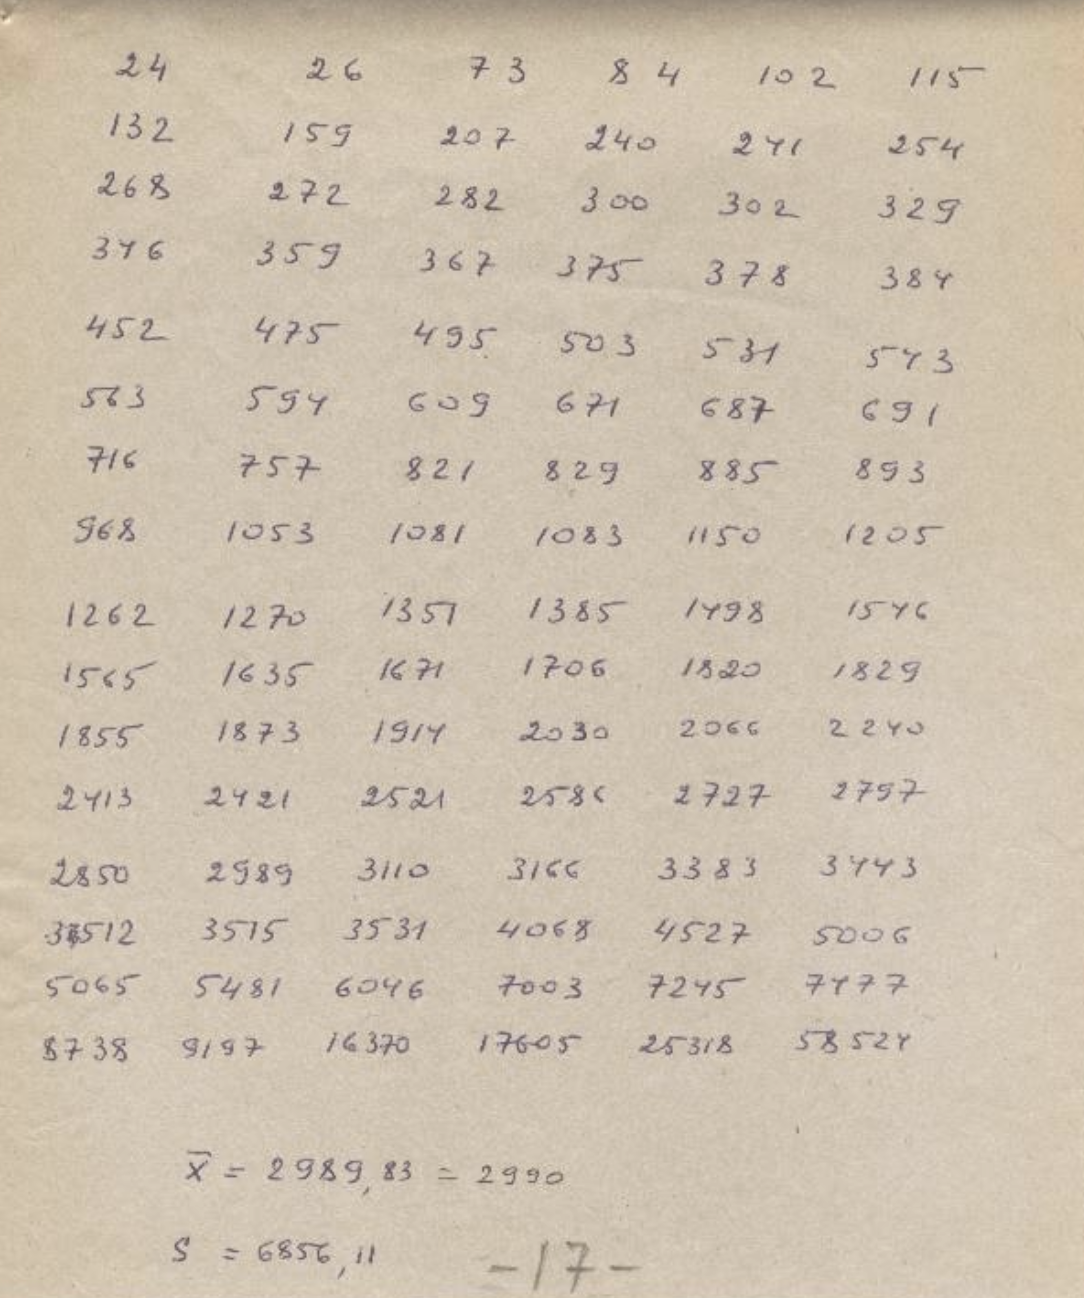
\includegraphics[scale=0.8]{pic1}
\caption{Таблица страховых возмещений}
\end{figure}



\begin{center}
	\begin{tabular}{ |c|c|c|c|c|c|} 
	 \hline
	 Стоим. возм. & набл.част. & теор.част.(эксп.) &  Pareto a) & Pareto b) & Weibull $W(c,\gamma)$ \\
	 \hline 
	 0-260 & 12 & 8 & 12.7 & 15.4 & 17.6 \\ 
	 \hline
	260 - 545 & 18 & 8 & 11.4 & 13.0 & 11.9 \\ 
	 \hline
	 545 - 860 & 10 & 8 & 10.2 & 10.9 & 10.0\\ 
	 \hline
	 860 - 1212 & 8 & 8 & 9.1 & 9.3 & 8.8 \\ 
	 \hline
	 1212 - 1612 & 7 & 8 & 8.2 & 8.0 & 7.9 \\ 
	 \hline
	 1612 - 2073 & 10 & 8 & 7.4 & 6.9 & 7.1 \\ 
	 \hline
	 2073 - 2618 & 5 & 8 & 6.7 & 6.0 & 6.5 \\ 
	 \hline
	 2618 - 3285 & 6 & 8 & 6.1 & 5.3 & 6.0 \\ 
	 \hline
	 3285 - 4145 & 6 & 8 & 5.6 & 4.8 & 5.5 \\ 
	 \hline
	 4145 - 5357 & 3 & 8 & 5.2 & 4.4 & 5.1 \\ 
	 \hline
	 5357 - 7430 & 4 & 8 & 5.1 & 4.2 & 4.8 \\ 
	 \hline
	 7430 - $\infty$ & 7 & 8 & 8.3 & 7.7 & 4.8 \\ 
	 \hline
	\end{tabular}
\end{center}


Строим гистограмму:

\begin{figure}[h!]
\centering
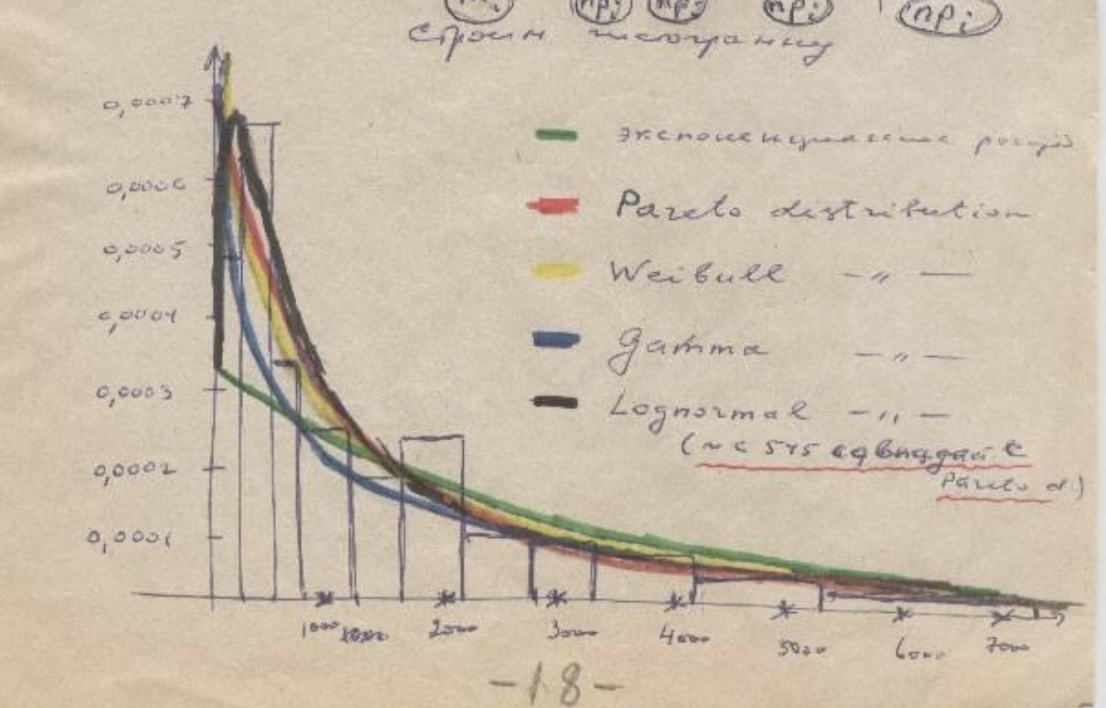
\includegraphics[scale=0.8]{pic2}
\caption{Гистограмма}
\end{figure}


Первоначальный общий вывод о типе распределения : оно ассиметричное с длинным хвостом.

\subsection{Экспоненциальное распределение} % (fold)
Пусть $\overline{\lambda} $ оценка параметра $\lambda$. Используя метод максимального правдоподобия , найдем, что
\[ \overline{\lambda} = \overline{X} = \frac{\sum X_i}{n}.\]

Для нашего случая $\overline{X} = 2990 = \overline{\lambda}. $

Проверяем гипотезу об экспоненциальном распределении с параметром $\overline{\lambda} = 2990  
.$

Проверяем с помощью критерия $\chi^2 = \sum\limits_{i=1}^{12}\frac{(m_i - np_i)^2}{np_i}$.

Весь интервал разбит на 12 интервалов, $m_i$ известны,$np_i$ подсчитываем. Получаем $\chi^2 = 23$ (у нас $\chi^2$ с 12 - 1 -1 = 10 степенями свободы). Тогда
\begin{gather*}
	\alpha = 0.01 \;\; \chi^2_{1-\alpha} = 23.2 \;\Rightarrow\;\; \text{ гипотеза отбрасывается}\\
	\alpha = 0.05 \;\; \chi^2_{1-\alpha} = 18.31
\end{gather*}

% subsection экспоненциальное_распределение (end)

% section распределения_потерь (end)
% section нетто_ставка_страхового_взноса (end)


% section апостериорное_распределение_числа_требований_на_t_t_ (end)
% section система_бонус_малус (end)
% subsection распределение_пуассона (end)
% section распределения_для_числа_страховых_требований (end)
% chapter лекция_6_страхование_не_жизни (end)

\end{document}
